%%%%%%%%%%%%%%%%%%%%%%%%%%%%%%%%%%%%%%%%%%%%%%%%%%%%%%%%%%%%%%%%%%%%%%%%%%%%%%%%
%% Plantilla de memoria en LaTeX para la EIF - Universidad Rey Juan Carlos
%%
%% Por Gregorio Robles <grex arroba gsyc.urjc.es>
%%     Grupo de Sistemas y Comunicaciones
%%     Escuela de Ingeniería de Fuenlabrada
%%     Universidad Rey Juan Carlos
%% (muchas ideas tomadas de Internet, colegas del GSyC, antiguos alumnos...
%%  etc. Muchas gracias a todos)
%%
%% La última versión de esta plantilla está siempre disponible en:
%%     https://github.com/gregoriorobles/plantilla-memoria
%%
%% Para obtener PDF, ejecuta en la shell:
%%   make
%% (las imágenes deben ir en PNG o JPG)

%%%%%%%%%%%%%%%%%%%%%%%%%%%%%%%%%%%%%%%%%%%%%%%%%%%%%%%%%%%%%%%%%%%%%%%%%%%%%%%%

\documentclass[a4paper, 12pt]{book}
%\usepackage[T1]{fontenc}

\usepackage[a4paper, left=2.5cm, right=2.5cm, top=3cm, bottom=3cm]{geometry}
\usepackage{times}
\usepackage[utf8]{inputenc}
\usepackage[spanish]{babel} % Comenta esta línea si tu memoria es en inglés
\usepackage{url}
%\usepackage[dvipdfm]{graphicx}
\usepackage{graphicx}
\usepackage{float}  %% H para posicionar figuras
\usepackage[nottoc, notlot, notlof, notindex]{tocbibind} %% Opciones de índice
\usepackage{latexsym}  %% Logo LaTeX
\usepackage{listings}

\title{Memoria del Proyecto}
\author{Nombre del autor}

\renewcommand{\baselinestretch}{1.5}  %% Interlineado

\begin{document}

\renewcommand{\refname}{Bibliografía}  %% Renombrando
\renewcommand{\appendixname}{Apéndice}


%%%%%%%%%%%%%%%%%%%%%%%%%%%%%%%%%%%%%%%%%%%%%%%%%%%%%%%%%%%%%%%%%%%%%%%%%%%%%%%%
% PORTADA

\begin{titlepage}
\begin{center}
\includegraphics[scale=0.6]{img/URJ_logo_Color_POS.png}

\vspace{1.75cm}

\LARGE
ESCUELA DE INGENIERÍA DE FUENLABRADA
\vspace{1cm}

\LARGE
INGENIERÍA EN SISTEMAS AUDIOVISUALES Y MULTIMEDIA

\vspace{1cm}
\LARGE
\textbf{TRABAJO FIN DE GRADO}

\vspace{2cm}

\Large
PLATAFORMA WEB PARA PROYECTOS DE ARQUITECTURA

\vspace{2cm}

\large
Autor : Bayas Pancho, Karol Joseth \\
Tutor : Robles Martínez, Gregorio\\
Cotutor: De Jorge Huertas, Virginia 
\vspace{1cm}

\large
Curso académico 202X/202X

\end{center}
\end{titlepage}

\newpage
\mbox{}
\thispagestyle{empty} % para que no se numere esta pagina



%%%%%%%%%%%%%%%%%%%%%%%%%%%%%%%%%%%%%%%%%%%%%%%%%%%%%%%%%%%%%%%%%%%%%%%%%%%%%%%%
%%%% Para firmar
\clearpage
\pagenumbering{gobble}
\chapter*{}

\vspace{-4cm}
\begin{center}
\LARGE
\textbf{Trabajo Fin de Grado}

\vspace{1cm}
\large
Plataforma WEB para Proyectos de Arquitectura

\vspace{1cm}
\large
\textbf{Autor :} Bayas Pancho, Karol Joseth \\
\textbf{Tutor :} Robles Martínez, Gregorio

\end{center}

\vspace{1cm}
La defensa del presente Proyecto Fin de Carrera se realizó el día \qquad$\;\,$ de \qquad\qquad\qquad\qquad \newline de 2024, siendo calificada por el siguiente tribunal:


\vspace{0.5cm}
\textbf{Presidente:}

\vspace{1.2cm}
\textbf{Secretario:}

\vspace{1.2cm}
\textbf{Vocal:}


\vspace{1.2cm}
y habiendo obtenido la siguiente calificación:

\vspace{1cm}
\textbf{Calificación:}


\vspace{1cm}
\begin{flushright}
Fuenlabrada, a \qquad$\;\,$ de \qquad\qquad\qquad\qquad de 202X
\end{flushright}

%%%%%%%%%%%%%%%%%%%%%%%%%%%%%%%%%%%%%%%%%%%%%%%%%%%%%%%%%%%%%%%%%%%%%%%%%%%%%%%%
%%%% Dedicatoria

\chapter*{}
\pagenumbering{Roman} % para comenzar la numeracion de paginas en numeros romanos
\begin{flushright}
\textit{Dedicado a \\
mi familia}
\end{flushright}

%%%%%%%%%%%%%%%%%%%%%%%%%%%%%%%%%%%%%%%%%%%%%%%%%%%%%%%%%%%%%%%%%%%%%%%%%%%%%%%%
%%%% Agradecimientos

\chapter*{Agradecimientos}
%\addcontentsline{toc}{chapter}{Agradecimientos} % si queremos que aparezca en el índice
\markboth{AGRADECIMIENTOS}{AGRADECIMIENTOS} % encabezado 

Con la finalizacion de este proyecto doy por finalizada mi etapa universitaris por lo que 
antetodo me gustaria presentar la gratitud que siento hacia los profesores de la ETSI. A 
lo largo de estos años, su orientación y sabiduría me han guiado en mi camino académico. 
En particular, quiero expresar mi sincero agradecimiento a Gregorio Robles, quien no solo nos 
introdujo en el mundo del desarrollo web, sino que también creyó en mí para la realización de 
este proyecto. Su constante disponibilidad para orientarme y su apoyo inquebrantable han sido invaluables.

También deseo expresar mi amor y gratitud hacia mi familia; a mis padres y hermanos que siempre han estado a mi lado. 
Su apoyo incondicional y constante ha sido mi roca en los momentos de dificultad. Sus palabras de aliento siempre me 
impulsaron a seguir adelante incluso cuando el camino era difícil. Su amor y apoyo han sido la columna vertebral de 
todos mis logros y por eso, estoy eternamente agradecido. 

Y a todos los que de alguna manera han contribuido a este trabajo, muchas gracias. Cada palabra de aliento, cada 
gesto de apoyo, ha sido fundamental para llegar hasta aquí. Este logro es tan suyo como mío.


%%%%%%%%%%%%%%%%%%%%%%%%%%%%%%%%%%%%%%%%%%%%%%%%%%%%%%%%%%%%%%%%%%%%%%%%%%%%%%%%
%%%% Resumen

\chapter*{Resumen}
%\addcontentsline{toc}{chapter}{Resumen} % si queremos que aparezca en el índice
\markboth{RESUMEN}{RESUMEN} % encabezado

Este proyecto es la culminación de mi grado en Ingeniería en Sistemas Audiovisuales y Multimedia, y es la construcción de una 
plataforma web diseñada especialmente para los amantes de la arquitectura. 

Usando el framework Flask de Python, la plataforma busca potenciar la colaboración y comunicación entre los estudiantes y profesores 
de arquitectura. La idea es proporcionar un espacio en el que los usuarios, ya sean estudiantes o profesores, puedan interactuar y 
compartir información relevante. Así, una vez estás registrado, puedes realizar varias tareas, como añadir eventos, libros, revistas, 
enlaces de interesantes y mucho más. 

La plataforma tiene a un administrador el cual tiene acceso a todas las partes del sistema y puede manejar la base de datos. 
De esta manera, si algo va mal o si necesitamos modificar algunos datos, el administrador puede hacerlo sin ningun problemas.

Además la plataforma permite la carga y gestión de archivos, incluyendo imágenes, videos, documentos PDF, entre otros. Estos 
archivos están a menudo vinculados a los libros de arquitectura presentes en la plataforma, proporcionando así una valiosa fuente de 
conocimiento e inspiración para cualquiera que esté interesado en el tema. 

Esta plataforma esta pensada para ser accesible desde cualquier navegador, por lo que puedes acceder a ella desde tu móvil, tableta o 
cualquier otro dispositivo. 

Cuenta además con diferentes tipos de usuarios por lo que si eres un alumno o un profesor, la plataforma te ofrece diferentes funcionalidades. 
Esto se hace para asegurar que cada usuario tenga una experiencia adaptada a sus necesidades y pueda aprovechar al máximo la plataforma.

En resumen, este proyecto no es solo una plataforma que facilita la colaboración entre alumnos y profesores. Es también 
una biblioteca virtual de conocimiento arquitectónico y una potente herramienta para mejorar la experiencia educativa en el 
campo de la arquitectura.

%%%%%%%%%%%%%%%%%%%%%%%%%%%%%%%%%%%%%%%%%%%%%%%%%%%%%%%%%%%%%%%%%%%%%%%%%%%%%%%%
%%%% Resumen en inglés

\chapter*{Summary}
%\addcontentsline{toc}{chapter}{Summary} % si queremos que aparezca en el índice
\markboth{SUMMARY}{SUMMARY} % encabezado

This project is the culmination of my degree in Audiovisual and Multimedia Systems Engineering, and it is the construction of a web 
platform designed especially for architecture enthusiasts.

Using the Flask framework of Python, the platform aims to enhance collaboration and communication among architecture students and 
professors. The idea is to provide a space where users, whether students or professors, can interact and share relevant information. 
Once registered, users can perform various tasks such as adding events or books, sharing interesting links, and much more.

The platform has an administrator who has access to all parts of the system and can manage the database. This way, if something goes 
wrong or if we need to modify something in the database, the administrator can do so without any issues.

Additionally, the platform allows for uploading and managing files, including images, videos, and PDF documents. These files are often 
linked to the architecture books present on the platform, thus providing a valuable source of knowledge and inspiration for anyone 
interested in the subject.

This platform is designed to be accessible from any browser, so you can access it from your mobile, tablet, or any other device.

It also has different types of users, so if you are a student or a teacher, the platform offers you different functionalities. This 
is done to ensure that each user has an experience tailored to their needs and can make the most out of the platform.

In summary, this project is not just a platform that facilitates collaboration between students and teachers. It is also a virtual 
library of architectural knowledge and a powerful tool to enhance the educational experience in the field of architecture.

%%%%%%%%%%%%%%%%%%%%%%%%%%%%%%%%%%%%%%%%%%%%%%%%%%%%%%%%%%%%%%%%%%%%%%%%%%%%%%%%
%%%%%%%%%%%%%%%%%%%%%%%%%%%%%%%%%%%%%%%%%%%%%%%%%%%%%%%%%%%%%%%%%%%%%%%%%%%%%%%%
% ÍNDICES %
%%%%%%%%%%%%%%%%%%%%%%%%%%%%%%%%%%%%%%%%%%%%%%%%%%%%%%%%%%%%%%%%%%%%%%%%%%%%%%%%

% Las buenas noticias es que los índices se generan automáticamente.
% Lo único que tienes que hacer es elegir cuáles quieren que se generen,
% y comentar/descomentar esa instrucción de LaTeX.

%%%% Índice de contenidos
\tableofcontents 
%%%% Índice de figuras
\cleardoublepage
%\addcontentsline{toc}{chapter}{Lista de figuras} % para que aparezca en el indice de contenidos
\listoffigures % indice de figuras
%%%% Índice de tablas
%\cleardoublepage
%\addcontentsline{toc}{chapter}{Lista de tablas} % para que aparezca en el indice de contenidos
%\listoftables % indice de tablas


%%%%%%%%%%%%%%%%%%%%%%%%%%%%%%%%%%%%%%%%%%%%%%%%%%%%%%%%%%%%%%%%%%%%%%%%%%%%%%%%
%%%%%%%%%%%%%%%%%%%%%%%%%%%%%%%%%%%%%%%%%%%%%%%%%%%%%%%%%%%%%%%%%%%%%%%%%%%%%%%%
% INTRODUCCIÓN %
%%%%%%%%%%%%%%%%%%%%%%%%%%%%%%%%%%%%%%%%%%%%%%%%%%%%%%%%%%%%%%%%%%%%%%%%%%%%%%%%

\cleardoublepage
\chapter{Introducción}
\label{sec:intro} % etiqueta para poder referenciar luego en el texto con ~\ref{sec:intro}
\pagenumbering{arabic} % para empezar la numeración de página con números

En el terreno educativo de la arquitectura, la colaboración eficiente y la comunicación fluida se están convirtiendo en elementos 
indispensables. Esta necesidad ha quedado plasmada en el proyecto que les presento hoy: una plataforma web construida con la finalidad 
de potenciar la interacción entre estudiantes y profesores del mundo arquitectónico.

La plataforma está diseñada para el intercambio de información relevante y facilitar la comunicación en torno a 
lo largo del calendario académico.

Promoviendo activamente la dinámica académica, este proyecto no es sólo una recopilación del conocimiento técnicos adquiridos durante 
el grado, sino que también representa un proyecto para mejorar la educación arquitectónica. 
\section{Estructura de la memoria}
\label{sec:seccion}

A continuación, se presenta una descripción de la estructura de la memoria, detallando el contenido de cada uno de los capítulos para 
proporcionar una guía organizada del trabajo de fin de grado:

\begin{itemize}
  \item \textbf{Capítulo 1: Introducción} \\
  En este capítulo, se presenta el contexto del trabajo, se define el problema de investigación y se destacan los objetivos del estudio. Además, se ofrece una breve descripción de la metodología utilizada y se justifica la relevancia del tema.
  \item \textbf{Capítulo 2: Objetivos del Proyecto} \\
  En este capítulo se proporciona información sobre los objetivos esperados del proyecto, las características que se pretende obtener y los objetivos esperados.  
  \item \textbf{Capítulo 3: Tecnologías Utilizadas} \\
  En este capítulo se proporciona información detallada sobre el diseño, las características y los usos de cada una de las tecnologías usadas en el proyecto.
  \item \textbf{Capítulo 4: Funcionamiento de la Aplicación} \\
  En este capítulo, se entra en detalle en el funcionamiento de la aplicación.
  \item \textbf{Capítulo 5: Experimentos y Pruebas} \\
  Se presentan los diferentes experimentos realizados y se prueba el correcto funcionamiento de la aplicación.
  \item \textbf{Capítulo 6: Resultados Obtenidos} \\
  En este capítulo, se explican los resultados obtenidos al poner a prueba varios aspectos de la aplicación.
  \item \textbf{Capítulo 7: Conclusiones} \\
  Se indican los resultados conseguidos y la solución a los objetivos no conseguidos.
\end{itemize}

\section{Motivación}
\label{sec:seccion}


En el trasfondo de la educación arquitectónica, me impulsa la firme convicción de que la tecnología puede desempeñar un papel transformador al mejorar la colaboración y la comunicación entre estudiantes y profesores. Inspirado por mis tutores Virginia y Gregorio en el deseo de superar las barreras existentes en la interacción educativa, he decidido emprender el desarrollo de esta plataforma web.

La motivación central detrás de esta iniciativa es la necesidad de proporcionar a la comunidad educativa de arquitectura una herramienta digital que simplifique y enriquezca su experiencia de aprendizaje. Observando las limitaciones en la comunicación y el intercambio de información, he visualizado esta plataforma como un espacio virtual donde la colaboración se vuelve intuitiva y donde la información relevante fluye de manera efectiva.

Con el objetivo de fomentar la participación activa, la plataforma busca ir más allá de ser simplemente un repositorio de datos. Pretende ser un medio dinámico donde los estudiantes pueden compartir ideas, los profesores pueden proporcionar orientación y todos pueden estar al tanto de los eventos educativos cruciales. La creación de esta plataforma no solo es un ejercicio técnico, sino una contribución tangible a la mejora de la calidad educativa en el ámbito de la arquitectura.

Creo firmemente que, al proporcionar un entorno digital eficiente y fácil de usar, esta plataforma puede marcar la diferencia, fomentando la comunicación. Esta motivación arraigada en la mejora continua y la innovación tecnológica impulsa mi dedicación a la creación de esta herramienta que aspira a enriquecer la experiencia educativa para estudiantes y profesores por igual.
\section{Objetivos e hipótesis de investigación}
\label{sec:seccion}

\subsection{Objetivos de Investigación}
\label{subsec:Objetivos de Investigación}

\begin{itemize}
  \item \textbf{Facilitar la Colaboración: } \\ 
  Se plantea la creación de un entorno digital diseñado específicamente para fomentar la colaboración entre estudiantes y profesores. Este entorno busca simplificar 
  y agilizar el intercambio de información y recursos educativos relevantes para la disciplina de la arquitectura. Se pretende que esta plataforma proporcione un 
  espacio donde los usuarios puedan compartir ideas, proyectos, documentos y otros materiales de forma eficiente, promoviendo así una mayor interacción y cooperación.
  \item \textbf{Centralizar Recursos: } \\ Se plantea el desarrollo de una plataforma digital que funcione como un repositorio centralizado para almacenar una 
  amplia variedad de recursos relacionados con la arquitectura. Esta plataforma tendría como objetivo principal mejorar tanto el acceso como la gestión de la 
  información educativa dentro del ámbito de la arquitectura. Al centralizar estos recursos, se facilitaría a estudiantes y profesores la búsqueda y el acceso a 
  libros, archivos y otros materiales relevantes para su formación y desarrollo académico. Además, se buscaría optimizar la organización y clasificación de estos 
  recursos para garantizar una experiencia de usuario fluida y eficiente.
  \item \textbf{Mejorar la Comunicación: } \\ Se propone la implementación de herramientas destinadas a mejorar la comunicación entre los usuarios de la plataforma. 
  Esto incluye la organización de eventos y la creación de foros de discusión, con el objetivo de fomentar una interacción más activa y un intercambio de ideas más 
  fluido entre los participantes. Estas herramientas permitirían a los usuarios compartir experiencias, plantear preguntas, discutir temas relevantes y colaborar en 
  proyectos de manera colaborativa. El enfoque está en promover una comunicación efectiva que enriquezca la experiencia educativa de los usuarios y fortalezca la 
  comunidad de aprendizaje en el ámbito de la arquitectura.
  \item \textbf{Optimizar la Experiencia del Usuario: } \\ Se plantea el diseño de una interfaz de usuario que sea intuitiva y fácil de usar, adaptada a las 
  necesidades particulares de los estudiantes y profesores del campo. El objetivo es mejorar significativamente la experiencia de navegación y participación 
  dentro de la plataforma. Se buscaría crear un entorno digital que sea accesible para usuarios de todos los niveles de habilidad tecnológica y que ofrezca 
  una experiencia fluida y agradable. Esto implica la implementación de un diseño claro y estructurado, la inclusión de funciones de búsqueda eficientes, 
  así como la disposición de herramientas y recursos relevantes de manera fácilmente accesible. \\ En resumen, se persigue la creación de un espacio digital 
  que potencie la interacción y el aprendizaje en el ámbito de la arquitectura mediante una experiencia de usuario óptima.
\end{itemize}

\subsection{Hipótesis de Investigación}
\label{subsec:Hipotesis de Investigacin}

\begin{itemize}
  \item \textbf{Mayor Colaboración:} \\ 
  Se espera que la implementación de la plataforma web fomente una mayor colaboración entre estudiantes y profesores al proporcionar un espacio digital diseñado 
  específicamente para compartir conocimientos y experiencias en el campo de la arquitectura. Esta colaboración promoverá un intercambio enriquecedor que contribuirá 
  al aprendizaje y al desarrollo profesional de los usuarios.
  \item \textbf{Eficiencia en la Gestión de Recursos:} \\ La centralización de recursos educativos, como libros, revistas, enlaces y archivos en la plataforma 
  facilitarán una gestión más eficiente y accesible de los materiales educativos para estudiantes y profesores. Al tener todos estos recursos disponibles en un único 
  lugar, los usuarios podrán acceder fácilmente a ellos, lo que mejorará significativamente su experiencia de aprendizaje y su capacidad para encontrar y utilizar 
  información relevante.
  \item \textbf{Mejora en la Comunicación:}\\ La introducción de herramientas de comunicación, como eventos y foros dentro de estos libros, fortalecerá la 
  comunicación entre los usuarios de la plataforma. Estas herramientas permitirán una interacción más activa y dinámica, facilitando la discusión de temas relevantes, 
  el intercambio de ideas y la colaboración en proyectos conjuntos. Esto contribuirá a crear una comunidad educativa más sólida y comprometida en el ámbito de la 
  arquitectura.
  \item \textbf{Aumento de la Participación:} \\La optimización de la experiencia del usuario en la plataforma resultará un aumento en la participación de los 
  usuarios. Al ofrecer una interfaz amigable, los usuarios se sentirán más cómodos y motivados para interactuar con la plataforma, lo que aumentará su compromiso 
  y su disposición a contribuir activamente al aprendizaje colaborativo y a la comunidad educativa en general.
\end{itemize}


%%%%%%%%%%%%%%%%%%%%%%%%%%%%%%%%%%%%%%%%%%%%%%%%%%%%%%%%%%%%%%%%%%%%%%%%%%%%%%%%
%%%%%%%%%%%%%%%%%%%%%%%%%%%%%%%%%%%%%%%%%%%%%%%%%%%%%%%%%%%%%%%%%%%%%%%%%%%%%%%%
% OBJETIVOS %
%%%%%%%%%%%%%%%%%%%%%%%%%%%%%%%%%%%%%%%%%%%%%%%%%%%%%%%%%%%%%%%%%%%%%%%%%%%%%%%%

\cleardoublepage % empezamos en página impar
\chapter{Objetivos} % título del capítulo (se muestra)
\label{chap:objetivos} % identificador del capítulo (no se muestra, es para poder referenciarlo)

\section{Objetivo general} % título de sección (se muestra)
\label{sec:objetivo-general} % identificador de sección (no se muestra, es para poder referenciarla)
El propósito de este proyecto es desarrollar un sistema de administración integral destinado a gestionar no solo libros y documentos, sino también eventos, revistas y enlaces de interés. El objetivo principal es mejorar significativamente la experiencia de los usuarios al proporcionar un acceso más fácil y eficiente a la información a través de una interfaz intuitiva y amigable. Para garantizar la seguridad y la privacidad de los usuarios, se implementarán funcionalidades como el inicio de sesión seguro y la opción de restablecimiento de contraseña en caso de olvido.

En esta plataforma, nos enfocamos en potenciar la interacción entre los usuarios para la gestión de eventos, la administración de libros y la exploración de revistas y enlaces relevantes. Además de estas funciones principales, hemos integrado herramientas administrativas que facilitarán a los usuarios la interacción de manera eficiente y efectiva con el sistema. Nuestro objetivo es crear una experiencia lo más amigable posible para todos los usuarios que utilicen este sistema, promoviendo una colaboración activa, una comunicación fluida y un acceso fácil a los recursos educativos y de interés en el campo de la arquitectura.

\section{Objetivos Específicos}
\label{sec:objetivos-especificos}

A continuación se detallan los objetivos específicos que guiarán el desarrollo y la implementación del sistema de administración:

\begin{enumerate}
  \item \textbf{Desarrollar Vistas de Administración:} \\Crear interfaces administrativas intuitivas y funcionales para la gestión de archivos, eventos y usuarios, proporcionando herramientas eficientes para realizar tareas de administración.
  \item \textbf{Desarrollar Vistas de Página Pública:} \\Diseñar una interfaz intuitiva y funcional que permita el acceso a la página web para cualquier persona, incluso si no forma parte de la comunidad registrada. Esta vista pública proporcionará una experiencia de navegación informativa y atractiva, sin acceso a funcionalidades de administración reservadas para usuarios registrados.
  \item \textbf{Implementar Sistema de Autenticación:} \\Desarrollar un sistema de autenticación robusto y seguro que permita el acceso protegido a las funcionalidades administrativas, garantizando la autenticidad y la autorización de los usuarios.
  \item \textbf{Diseñar Páginas de Visualización:} \\Diseñar páginas de visualización atractivas y de fácil navegación para la presentación de libros, eventos y comentarios, asegurando una experiencia de usuario óptima para todos los usuarios.
  \item \textbf{Integrar Sistema de Comentarios:} \\Incorporar un sistema de comentarios interactivo que permita a los usuarios expresar sus opiniones y compartir comentarios sobre los libros, fomentando la participación y el intercambio de ideas.
  \item \textbf{Gestionar Eventos:} \\Implementar funciones de gestión de eventos que posibiliten la visualización, edición y organización eficiente de eventos, proporcionando información relevante y actualizada.
  \item \textbf{Administrar Libros:} \\Desarrollar funcionalidades completas para la gestión de libros, incluyendo la capacidad de agregar, editar y eliminar libros, así como la asociación adecuada con los autores correspondientes.
  \item \textbf{Administrar Enlaces y Revistas:} \\Implementar funcionalidades para la gestión de revistas y enlaces, que permitan a los usuarios agregar y eliminar tanto revistas como enlaces de interés
  \item \textbf{Implementar Herramientas Administrativas:} \\Integrar herramientas administrativas avanzadas para la gestión de usuarios, roles y permisos, permitiendo una administración eficaz y segura del sistema.
  \item \textbf{Optimizar la Seguridad:} \\Mejorar la seguridad del sistema mediante la implementación de técnicas avanzadas de almacenamiento y recuperación de contraseñas, garantizando la protección de la información confidencial.
  \item \textbf{Aplicar Restricciones de Acceso:} \\Establecer restricciones de acceso basadas en roles para controlar qué usuarios pueden acceder a determinadas funcionalidades, asegurando un uso adecuado y autorizado del sistema.
  \item \textbf{Garantizar la Integridad de los Datos:} \\Implementar medidas para asegurar la integridad de los datos almacenados en la base de datos, evitando inconsistencias y errores que puedan comprometer la fiabilidad y la precisión de la información.
\end{enumerate}

Estos objetivos específicos serán clave para el desarrollo exitoso del sistema de administración, garantizando su funcionalidad, seguridad y eficiencia en la gestión de recursos y usuarios.

\section{Planificación temporal}
\label{sec:planificacion-temporal}
La ejecución de este proyecto de Trabajo de Fin de Grado correspondió a un período de ocho meses, desde julio de 2023 hasta febrero de 2024. A continuación, un breve desglose de la planificación temporal del proyecto:

\begin{figure}
  \centering
  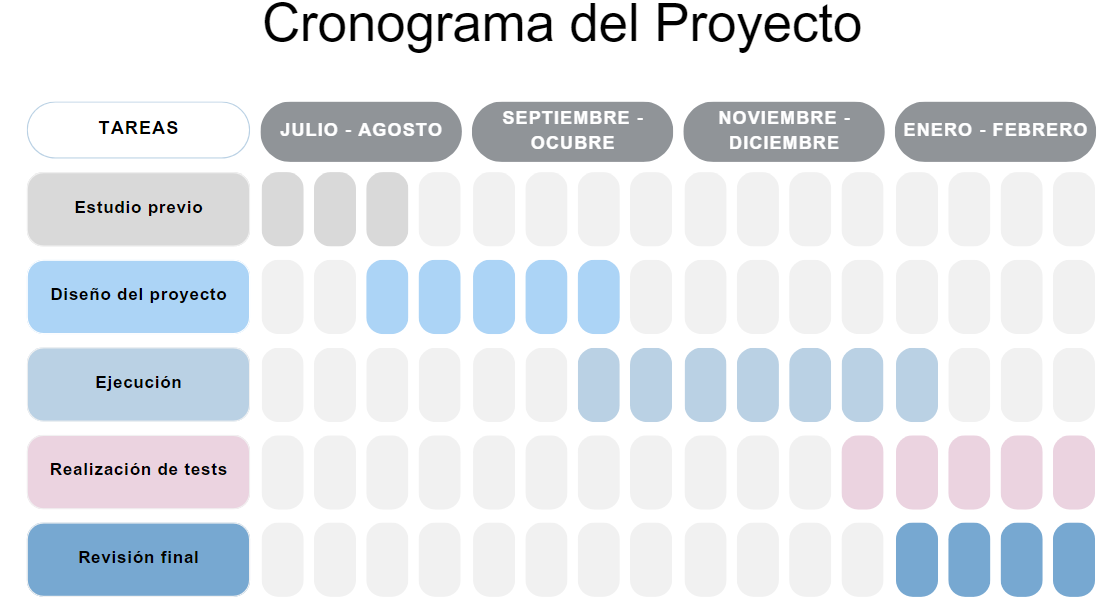
\includegraphics[width=0.7\textwidth]{img/gann.png}
  \caption{Diagrama de Gantt}
  \label{fig:arquitectura}
\end{figure}

\begin{itemize}
  \item \textbf{Julio 2023: } Este mes marca el inicio del proyecto, con la presentación del mismo bajo la guía del profesor Gregorio Robles Martínez. Además, comienzan las reuniones con Virginia, mi codirectora de Trabajo de Fin de Grado (TFG), donde juntos empezamos a esbozar los elementos básicos que queríamos incorporar en el sitio web.
  \item \textbf{Agosto 2023: } Dediqué este mes a una serie de consultas repetidas con Virginia para afinar la visión del proyecto. Realizamos una exploración exhaustiva de diversas páginas web centradas en arquitectura, con el objetivo de infundir ideas innovadoras en nuestra propia plataforma.
  \item \textbf{Agosto - Octubre 2023: } Durante este período, estuve completamente inmerso en la fase de implementación y desarrollo de la plataforma web. Construí páginas dedicadas tanto para usuarios registrados como para visitantes. Durante las sesiones tutoriales, nos centramos en aspectos técnicos como el manejo de permisos de usuarios, la incorporación de un sistema de admisión de usuarios y la funcionalidad de recuperación de contraseñas.
  \item \textbf{Noviembre - Diciembre 2023: } Durante estos meses, se llevaron a cabo importantes adiciones a la plataforma. Integré un calendario y una sección de libros para enriquecer la experiencia del usuario. Además, se habilitaron los comentarios, aunque solo para usuarios registrados, con el fin de fomentar la participación y el intercambio de ideas.
  \item \textbf{Enero - Febrero 2024: } Durante los últimos dos meses, nos reunimos para finalizar detalles pendientes y abordar los últimos requisitos del proyecto. Además, comenzamos a redactar la memoria del proyecto y corregimos ciertos detalles en el código según las necesidades identificadas. Este período fue crucial para garantizar la calidad y la coherencia del trabajo realizado antes de su presentación final.
\end{itemize}


%%%%%%%%%%%%%%%%%%%%%%%%%%%%%%%%%%%%%%%%%%%%%%%%%%%%%%%%%%%%%%%%%%%%%%%%%%%%%%%%
%%%%%%%%%%%%%%%%%%%%%%%%%%%%%%%%%%%%%%%%%%%%%%%%%%%%%%%%%%%%%%%%%%%%%%%%%%%%%%%%
% ESTADO DEL ARTE %
%%%%%%%%%%%%%%%%%%%%%%%%%%%%%%%%%%%%%%%%%%%%%%%%%%%%%%%%%%%%%%%%%%%%%%%%%%%%%%%%

\cleardoublepage
\chapter{Estado del arte}
\label{chap:estado}

En este capítulo se presentarán las herramientas y librerías utilizadas en el Trabajo de Fin de Grado. Esto nos proporcionará una visión detallada de las tecnologías empleadas a lo largo del proyecto, lo cual es fundamental para comprender la infraestructura y el entorno de desarrollo utilizados en la implementación de la plataforma.

\section{Tecnologías y Herramientas}
\label{sec:tecnologias y herramientas}

\subsection{Python} 
\label{subsec:Python} 
Python\footnote{\url{https://www.python.org/}}, desarrollado por Guido van Rossum a finales de los 80 en los Países Bajos, es un lenguaje 
de programación con un enfoque en la legibilidad del código y la productividad del programador. Desde su primera versión en 1991, ha 
experimentado un crecimiento significativo y se ha convertido en uno de los lenguajes más populares y utilizados en la actualidad. Su sintaxis simple, 
clara y precisa facilita la escritura de código limpio, mientras que su extensa gama de bibliotecas estándar acelera el proceso de desarrollo. 
Su adaptabilidad y compatibilidad con diversos paradigmas de programación han permitido su uso en una amplia variedad de aplicaciones, desde el 
desarrollo de software hasta el análisis de datos y machine learning.

\subsection{GitHub} 
\label{subsec:github} 
GitHub \footnote{\url{https://github.com/}} es un servicio en la nube que aloja un sistema de control de versiones, Git, lo que permite a los 
desarrolladores colaborar en proyectos compartidos manteniendo un seguimiento detallado de su progreso. Funciona como una plataforma web para el 
desarrollo colaborativo de software, facilitando la colaboración y el almacenamiento de proyectos de código abierto o privado. En GitHub, los usuarios 
pueden trabajar juntos en proyectos, compartiendo ideas y soluciones. Su principal ventaja es la posibilidad de trabajar en un proyecto en cualquier 
lugar y momento, ya que se realiza un seguimiento del desarrollo de forma remota. Además, proporciona otras funciones vitales a los desarrolladores, 
como bibliotecas y funciones para la gestión de versiones de software, la gestión de problemas y la revisión de código.\cite{tfg-karol}

\subsection{PHPMyAdmin}
\label{subsec:phpmyadmin} 
PHPMyAdmin\footnote{\url{http://localhost/phpmyadmin/}} es una herramienta creada en PHP que facilita la administración de bases de datos 
MySQL a través de una interfaz de usuario en un navegador web. 
Entre sus funciones se incluyen:\cite{phpmyadmin} la creación, modificación y eliminación de bases de datos y tablas; la gestión de campos y el ajuste de privilegios; y la 
capacidad de exportar datos en varios formatos. Esta herramienta multilingüe está disponible bajo la licencia GPL Versión 2. Desde su creación en 1998, 
PHPMyAdmin ha experimentado continuos avances y adaptaciones a las máquinas con servidores web y soporte de PHP y MySQL.

\subsection{JavaScript}
\label{subsec:JavaScript} 
JavaScript\footnote{\url{https://lenguajejs.com/javascript/}} es un lenguaje de programación de alto nivel, interpretado y orientado a objetos, conocido por su capacidad para ofrecer 
interactividad a las páginas web. Es un lenguaje del lado del cliente, por lo que se ejecuta en el navegador del usuario y puede interactuar con el contenido 
de la página, el Document Object Model (DOM) y otros elementos del navegador. Puede manipular el contenido de la página y responder a eventos del usuario. 
Además, es un lenguaje asincrónico, lo que le permite realizar tareas sin bloquear la ejecución del código. Es esencial para la manipulación del DOM, permitiendo 
agregar, eliminar o modificar elementos dinámicamente. También maneja eventos del usuario, facilita la creación de aplicaciones web interactivas y utiliza 
tecnologías como XMLHttpRequest o la interfaz Fetch para realizar solicitudes asíncronas al servidor. Dispone de diversos frameworks y bibliotecas que facilitan 
el desarrollo de aplicaciones web complejas. Además, sigue las especificaciones definidas por ECMAScript y es pluriparadigmático, admitiendo varios estilos de 
programación.

\subsection{Docker}
\label{subsec:Docker}
Docker\footnote{\url{https://www.docker.com/}} es una plataforma de código abierto que permite automatizar el despliegue, la escalabilidad y la operación de 
aplicaciones dentro de contenedores de software. Estos contenedores permiten empaquetar una aplicación junto con todas sus dependencias en una unidad estandarizada 
para el desarrollo de software, lo que facilita su portabilidad entre distintos entornos.

Algunos de los puntos clave de Docker son:

\begin{enumerate}
  \item \textbf{Portabilidad:} Docker permite empaquetar y ejecutar aplicaciones en prácticamente cualquier entorno, lo que facilita la migración de aplicaciones y sistemas.
  \item \textbf{Aislamiento:} Los contenedores de Docker permiten el aislamiento de recursos, lo que garantiza que cada contenedor funcione como una unidad autónoma y que los problemas en un contenedor no afecten a otros.
  \item \textbf{Eficiencia:} Docker es muy eficiente en términos de rendimiento ya que los contenedores que utiliza consumen menos recursos que las máquinas virtuales equivalentes.
  \item \textbf{Escalabilidad:} Docker facilita la escalabilidad de las aplicaciones, ya que permite crear y desplegar contenedores rápidamente y en gran medida.
  \item \textbf{Integración continua y entrega continua (CI/CD):} Docker se integra bien con los sistemas de CI/CD, lo que permite probar las aplicaciones en contenedores en distintas etapas del desarrollo y despliegue de forma automatizada.
  \item \textbf{Descentralización del desarrollo:} Docker ayuda a los equipos de desarrollo a trabajar de manera descentralizada y colaborativa, ya que cualquier miembro del equipo puede crear y desplegar contenedores con su propio trabajo. 
\end{enumerate}

\subsection{LaTeX}
\label{subsec:LaTeX}
LaTeX\footnote{\url{https://es.overleaf.com/}} es un sistema de composición de textos basado en TeX, desarrollado por Leslie Lamport en 1984, que automatiza la generación de documentos científicos, técnicos y académicos de alta calidad. Al aprovechar las funciones avanzadas de TeX, LaTeX permite crear documentos con una amplia variedad de elementos, como fórmulas matemáticas, imágenes y texto programático, utilizando una sintaxis de comandos para controlar la estructura y el formato del documento. Ampliamente utilizado en la comunidad científica y académica debido a su capacidad para producir documentos profesionales con facilidad y eficiencia, LaTeX es una herramienta esencial para la creación de contenido complejo y detallado.

\section{Liberías}
\label{sec:Librerias}

En el proyecto se emplearon diversas tecnologías para desarrollar una plataforma web robusta y escalable. Se utilizó HTML, CSS y JavaScript para la interfaz de usuario, Bootstrap y jQuery para el diseño y la funcionalidad, Flask en el lado del servidor con Python para la lógica y la gestión de la base de datos, MySQL y phpMyAdmin para la gestión de la base de datos, y Git para el control de versiones del código. Estas herramientas permitieron cumplir con los requisitos del proyecto de manera efectiva.
\subsection{Flask} 
\texttt{from flask import Blueprint, render\_template, redirect, session, request, flash, url\_for} Flask\cite{flaskbook}es un marco de trabajo para desarrollo web en Python. Las funciones mencionadas son partes esenciales de Flask:

\begin{itemize}
  \item \texttt{Blueprint}: Permite organizar rutas en módulos separados para una mejor organización del código.
  \item \texttt{render\_template}: Se utiliza para renderizar archivos de plantillas y generar una respuesta HTTP a partir de ellos.
  \item \texttt{redirect}: Redirige al navegador a otra URL.
  \item \texttt{session}: Permite almacenar información que es persistente entre las solicitudes, como datos de usuario.
  \item \texttt{request}: Proporciona información sobre la solicitud HTTP del cliente, como parámetros de formulario.
  \item \texttt{flash}: Se usa para enviar mensajes a la próxima solicitud, lo que resulta útil para proporcionar feedback al usuario.
  \item \texttt{url\_for}: Genera una URL a una vista basada en un nombre y argumentos, lo que facilita la generación de enlaces dinámicos.
\end{itemize}

\subsection{Flask-Mail}
\texttt{from flask\_mail import Message} Flask-Mail es una extensión que facilita el envío de correos electrónicos desde una aplicación Flask. Permite crear y enviar mensajes de correo electrónico de manera sencilla.

\subsection{Werkzeug}
\texttt{from werkzeug.utils import secure\_filename} Werkzeug es una biblioteca WSGI utilizada en Flask. \texttt{secure\_filename} se utiliza para asegurar que los nombres de archivo proporcionados por los usuarios sean seguros para usar en el sistema de archivos, evitando posibles ataques de inyección de directorios.

\subsection{mysql-connector-python}
\texttt{from config import mysql, mail} Esta biblioteca es la implementación oficial de MySQL para Python. Proporciona un conjunto de operaciones de base de datos y manejo de errores compatibles con el estándar DB API. En este caso, \texttt{mysql} es una instancia de conexión a la base de datos MySQL configurada en un archivo de configuración (\texttt{config.py}), que se importa para interactuar con MySQL en la aplicación Flask.

\subsection{os, random, string}
\texttt{import os, random, string} Estos son módulos estándar de Python:
\begin{itemize}
  \item \texttt{os}: Proporciona una manera de utilizar funcionalidades dependientes del sistema operativo, como la manipulación de archivos.
  \item \texttt{random}: Se utiliza para generar números aleatorios o seleccionar elementos aleatorios de una secuencia.
  \item \texttt{string}: Contiene operaciones comunes para trabajar con cadenas de texto, como la generación de caracteres aleatorios.
\end{itemize}

\subsection{Decorators y Config}
\texttt{decorators} y \texttt{config} son módulos personalizados creados específicamente para la aplicación. 
\begin{itemize}
  \item \texttt{config}: Contiene configuraciones de la aplicación, como la cadena de conexión a la base de datos y otras variables de entorno.
  \item \texttt{decorators}: Contiene decoradores personalizados que se utilizan en las vistas para agregar funcionalidades adicionales, como la autenticación de usuarios.
\end{itemize}

\subsection{Flask-Login}
\label{subsec:flasklogin} 
Flask-Login es una extensión de Flask que proporciona funcionalidades relacionadas con la gestión de sesiones de usuarios. 
Ofrece funciones esenciales para manejar la autenticación de usuarios, tales como iniciar sesión, cerrar sesión, recordar usuarios y proteger ciertas 
vistas para que solo los usuarios autenticados puedan acceder a ellas.

\subsection{Flask-MySQL y Flask-MySQLdb} 
\label{subsec:flaskmysqldb} 
Flask-MySQL y Flask-MySQLdb son extensiones de Flask que proporcionan soporte para MySQL en aplicaciones de Flask. Estas bibliotecas facilitan la interacción con bases de datos MySQL.

\subsection{MySQLClient y PyMySQL} 
\label{subsec:pymysql} 
MySQLClient y PyMySQL son interfaces de Python para conectarse con MySQL y realizar operaciones en la base de datos.
\subsection{FullCalendar}
\label{subsec:fullcalendar}
FullCalendar es una potente librería de JavaScript que permite crear calendarios interactivos y personalizables para aplicaciones web. 
Esta librería ha sido desarrollada para facilitar la visualización y gestión de eventos en calendarios en entornos web, ofreciendo una 
gran variedad de características y opciones de configuración.

\subsection{Itsdangerous} 
\label{subsec:itsdangerous} 
Itsdangerous es una biblioteca de Python que se utiliza para garantizar la seguridad en las aplicaciones. Proporciona varios ayudantes para pasar datos de manera segura.

\subsection{MarkupSafe} 
\label{subsec:markupsafe} 
MarkupSafe es una biblioteca de Python que se utiliza para crear cadenas seguras para usar en HTML y XML.
\subsection{Flask-Mail}
\label{subsec:flaskmail} 
Flask-Mail es una extensión de Flask que simplifica el envío de correos desde aplicaciones de Flask. Proporciona una interfaz sencilla 
para la configuración de correos y envío de mensajes, facilitando la implementación de funcionalidades relacionadas con correos, como la confirmación de cuentas 
o la recuperación de contraseñas.
\subsection{Pip} 
\label{subsec:pip} 
Pip es un sistema de administración de paquetes para Python y se utiliza para instalar y administrar paquetes de software escritos en Python.
\subsection{Jinja2}
\label{subsec:jinja2} 
Jinja2 es un motor de plantillas para Python que permite la generación de contenido HTML dinámico. Se utiliza en conjunto con Flask para 
generar páginas web dinámicas y se distingue por su simplicidad y flexibilidad. 

Algunas características clave de Jinja2:

\begin{enumerate}
  \item \textbf{Sintaxis de plantillas:} Jinja2 proporciona una sintaxis clara y concisa para la definición de plantillas, permitiendo a los desarrolladores generar 
  contenido dinámico de manera eficiente y legible.
  \item \textbf{Herencia de plantillas:} Permite la reutilización de código a través de la herencia de plantillas, donde una plantilla puede heredar bloques de contenido 
  de una plantilla padre.
  \item \textbf{Filtros:} Proporciona una serie de filtros útiles que transforman variables para su visualización. Algunos ejemplos son filtros para cambiar a mayúsculas 
  o minúsculas, truncar texto, modificar fechas, entre otros.
  \item \textbf{Tags de control de flujo:} Ofrece tags para estructuras de control, como bucles y condicionales. Con ellos, es posible realizar operaciones como recorrer 
  listas o verificar condiciones para mostrar u ocultar partes de la plantilla.
  \item \textbf{Escapado de texto:} Se encarga automáticamente del escapado de texto, protegiendo las aplicaciones de ataques como Cross Site Scripting (XSS).
  \item \textbf{Alto rendimiento:} Compila las plantillas en bytecode de Python, lo que significa que la ejecución de las plantillas es rápida y eficiente.
\end{enumerate}

En el código HTML, Jinja2 se utiliza para incluir fragmentos de código HTML con la directiva \texttt{include}, para iterar sobre rangos de números con la directiva 

\texttt{for}, y para insertar valores de variables con las llaves dobles (\texttt{{\{ variable \}}}).

\subsection{MySQL}
\label{subsec:mysql} MySQL\footnote{https://www.mysql.com/} es un sistema de gestión de bases de datos relacional (RDBMS) de código abierto que utiliza el lenguaje de consulta estructurado (SQL) 
para manipular datos. Destaca por su escalabilidad para adaptarse de aplicaciones pequeñas a sistemas empresariales de gran tamaño, su soporte para transacciones, 
su compatibilidad con diversas plataformas, y su robusta comunidad de usuarios. Ofrece diferentes motores de almacenamiento, siendo InnoDB uno de los más populares 
por su soporte de transacciones ACID. Asimismo, proporciona variadas herramientas y utilidades para la administración y monitoreo de bases de datos.


\subsection{Bootstrap}
\label{subsec:bootstrap} Bootstrap\footnote{https://getbootstrap.com/} es un framework de desarrollo frontend basado en HTML, CSS y JavaScript, que facilita la creación de interfaces web responsivas. 
Proporciona un sistema de rejilla para organizar el diseño en filas y columnas, un conjunto de componentes predefinidos reutilizables (botones, formularios, navegación, 
alertas, etc.), estilos predeterminados para la tipografía y funcionalidades interactivas mediante JavaScript. Aunque ofrece un conjunto completo de estilos y 
componentes, Bootstrap es altamente personalizable. Cuenta con una documentación detallada y una amplia comunidad de desarrolladores.

\subsection{jQuery}
\label{subsec:jquery}
jQuery es una biblioteca de JavaScript ampliamente utilizada que proporciona una forma simplificada de manipular el DOM, manejar eventos, crear animaciones y realizar llamadas AJAX. Es reconocida por su facilidad de uso y su soporte multiplataforma. 

Las características claves de jQuery son las siguientes:

\begin{enumerate}
  \item \textbf{Manipulación del DOM:} jQuery proporciona una interfaz fácil y eficiente para manipular el árbol de elementos DOM en una página web.
  \item \textbf{Facilidad de uso:} jQuery presenta una API fácil de usar que funciona en una multitud de navegadores. Esto incluye una manera sencilla de navegar por un documento, crear animaciones, manejar eventos y desarrollar aplicaciones con AJAX.
  \item \textbf{Llamadas AJAX:} jQuery simplifica mucho el proceso de envío de solicitudes AJAX y la manipulación de las respuestas.
  \item \textbf{Compatibilidad entre navegadores:} jQuery es conocida por manejar de manera eficiente muchas de las incompatibilidades entre diferentes versiones de navegadores y sus respectivos motores de JavaScript.
  \item \textbf{Extensibilidad:} jQuery puede ser extendida de diversas maneras para crear, por ejemplo, nuevos métodos que pueden ser reutilizados en más de un proyecto jQuery.
\end{enumerate}

En el código proporcionado se utiliza jQuery para ejecutar una serie de funciones después de que el documento HTML esté cargado y listo. 

\begin{verbatim} 
    $(document).ready(function(){/código/});
\end{verbatim}

Además, se utiliza para localizar elementos en el DOM, vincular eventos a elementos, enviar solicitudes AJAX y manipular la interfaz del usuario.

\subsection{Google Translate API}
\label{subsec:google_translate_api}
La API de Google Translate se utiliza para integrar la funcionalidad de traducción en aplicaciones, sitios web, y servicios. Esta API permite la traducción de texto en tiempo 
real a varios idiomas y se basa en los mismos algoritmos de aprendizaje automático que utiliza Google Translate. 

Las características claves de Google Translate API son:

\begin{enumerate}
  \item \textbf{Detección de idioma:} La API puede detectar automáticamente el idioma de la entrada y traducirlo al idioma de la salida requerido.
  \item \textbf{Diversidad de idiomas:} Soporta más de 100 idiomas.
  \item \textbf{Traducción en tiempo real:} Permite la traducción de texto en tiempo real, lo que permite a los usuarios obtener traducciones instantáneas mientras escriben.
  \item \textbf{Simplicidad de uso:} Con solo algunas líneas de código, los desarrolladores pueden integrar fácilmente la API en sus aplicaciones o sitios web.
\end{enumerate}

En el archivo "translation.js", Google Translate API se utiliza para inicializar un nuevo objeto de traducción con una configuración específica y para traducir el contenido de una página a un idioma especificado.

%%%%%%%%%%%%%%%%%%%%%%%%%%%%%%%%%%%%%%%%%%%%%%%%%%%%%%%%%%%%%%%%%%%%%%%%%%%%%%%%
%%%%%%%%%%%%%%%%%%%%%%%%%%%%%%%%%%%%%%%%%%%%%%%%%%%%%%%%%%%%%%%%%%%%%%%%%%%%%%%%
% DISEÑO E IMPLEMENTACIÓN %
%%%%%%%%%%%%%%%%%%%%%%%%%%%%%%%%%%%%%%%%%%%%%%%%%%%%%%%%%%%%%%%%%%%%%%%%%%%%%%%%

\cleardoublepage
\chapter{Diseño e implementación}
\label{sec:diseno}

A continuación, se expondrán con detalle los métodos y herramientas empleados en la ejecución del proyecto, ofreciendo una perspectiva minuciosa sobre el desarrollo 
de la iniciativa que tiene como finalidad la creación de una página web para el almacenamiento de toda la documentación relevante. Este capítulo ahonda en las diversas 
etapas del proyecto, detallando las decisiones adoptadas y las justificaciones vinculadas a las metodologías seleccionadas. 
Asimismo, se expone el diseño e implementación del proyecto con la intención de proporcionar a otros la capacidad de contribuir, adaptar o ampliar el sistema. 
Esta sección brinda una visión completa de cómo se estructuró y llevó a cabo el proyecto, abarcando las distintas fases de su creación.


\section{Arquitectura general} 
\label{sec:arquitectura}

En esta sección, es examinada en detalle la arquitectura general del proyecto. La organización de los archivos y directorios tiene un propósito específico que soporta 
la funcionalidad, el mantenimiento, y la escalabilidad del proyecto. Entender esta estructura facilita navegar por el código y contribuye al desarrollo del proyecto.

La estructura del proyecto se describe a continuación:

\begin{figure}
  \centering
  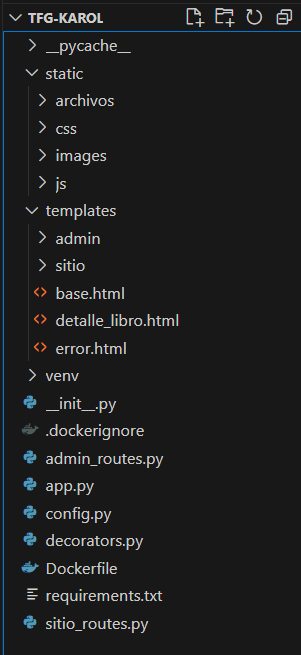
\includegraphics[width=0.25\textwidth]{img/estructura.png}
  \caption{Estructura del proyecto}
  \label{fig:estructura}
\end{figure}

\begin{itemize}
  \item \texttt{static/}: En este directorio se encuentran los archivos estáticos que son solicitados directamente por el cliente, como las hojas de estilo CSS, los scripts JavaScript, las imágenes, archivos y otros recursos multimedia. Esto permite una carga rápida y eficiente de los elementos visuales de la aplicación en el navegador del usuario.
  \item \texttt{templates/}: Aquí residen las plantillas HTML utilizadas por Flask para generar las páginas web dinámicas. Estas plantillas incluyen el código HTML junto con expresiones y directivas específicas de Flask que permiten la inserción de datos dinámicos en las páginas. Separar las plantillas del código Python facilita la gestión del contenido y la presentación de la aplicación.
  \item \texttt{venv/}: Este directorio alberga el entorno virtual de Python utilizado para instalar y gestionar las dependencias del proyecto. El uso de un entorno virtual garantiza que las dependencias del proyecto se instalen de forma aislada, evitando conflictos con otras versiones de paquetes instalados globalmente en el sistema.
  \item \texttt{\_init\_.py}: Este archivo especial indica a Python que el directorio debe tratarse como un paquete. Aunque puede estar vacío, comúnmente se utiliza para inicializar el paquete o para importar funciones y clases que se utilizarán en otros módulos del proyecto.
  \item \texttt{admin\_routes.py, sitio\_routes.py}: Estos módulos definen las rutas de la aplicación, que asignan las URL a las funciones encargadas de manejar las solicitudes del cliente. Separar las rutas en distintos archivos según su funcionalidad ayuda a mantener el código organizado y facilita su mantenimiento y escalabilidad.
  \item \texttt{app.py}: Este archivo sirve como punto de entrada de la aplicación Flask. Aquí se inicializa la aplicación Flask y se integran los distintos componentes del proyecto, como las rutas, las configuraciones y las extensiones. Es el archivo principal que ejecuta la aplicación y gestiona su funcionamiento.
  \item \texttt{config.py}: Contiene los valores de configuración de la aplicación, como las claves secretas y la información de conexión a la base de datos. Separar la configuración en un archivo dedicado facilita su gestión y permite ajustar la configuración según el entorno de desarrollo, pruebas o producción.
  \item \texttt{decorators.py}: En este archivo se definen los decoradores personalizados utilizados en el proyecto. Los decoradores son funciones que envuelven otras funciones y permiten agregar funcionalidades adicionales, como la autenticación de usuarios o el control de acceso. Su uso ayuda a mantener el código limpio y modular, facilitando la implementación de políticas de seguridad y autorización.
  \item \texttt{Dockerfile}: Contiene las instrucciones para construir una imagen Docker de la aplicación. Docker es una herramienta de virtualización que permite encapsular la aplicación y todas sus dependencias en un contenedor independiente, lo que facilita su despliegue en diferentes entornos de producción de manera consistente y reproducible.
  \item \texttt{requirements.txt}: En este archivo se listan todas las dependencias de Python necesarias para ejecutar el proyecto. Estas dependencias pueden instalarse fácilmente utilizando la herramienta pip, lo que simplifica la gestión de las dependencias y garantiza que todas las bibliotecas necesarias estén disponibles en el entorno de ejecución.
\end{itemize}

Esta estructura organizada y coherente de archivos y directorios ayuda a mantener separados los distintos aspectos de la aplicación, facilitando su desarrollo, mantenimiento y escalabilidad a medida que el proyecto evoluciona.
\section{Arquitectura específica} 
\label{sec:arquitectura}

\subsection{Programa principal}
\label{subsec:programaprincipal}

El archivo \texttt{app.py} es el que inicializa la aplicación Flask y con el cual se establece la configuración principal de la misma. Las configuraciones incluyen la conexión a la base de datos 
MySQL, la inicialización del correo y la generación de una clave secreta para la sesión.
Con el fin de proveer mayor seguridad, se implementa un decorador \texttt{login\_required}, el cual se encarga de verificar si el usuario ha iniciado sesión antes de 
poder acceder a ciertas rutas.

A continuación, se encuentran varias rutas esenciales del proyecto con sus respectivas funciones de manejo:

\begin{itemize}
   \item \texttt{/}: Redirige al usuario a la página principal.
   \item \texttt{/ver\_libro()}: Con esta función se puede visualizar el detalle de cada libro, la función realiza una consulta a la base de datos para obtener la 
   información específica de un libro. También se manejan los errores en caso de no encontrar el libro en cuestión.
   \item \texttt{/update\_event()}: Esta ruta se utiliza para actualizar los detalles de un evento específico, donde se recogen los datos del evento a través de una 
   consulta POST y se actualizan en la base de datos.
   \item \texttt{/insert\_event()}: Esta función maneja la inserción de un nuevo evento en la base de datos al recibir la información relevante del evento a través de una consulta POST.
   \item \texttt{/ajax\_delete()}: Esta función realiza la eliminación de un evento específico cuando se recibe una solicitud POST que contiene el id del evento a eliminar.
\end{itemize}

Finalmente, el registro de los blueprints se realiza al final. Los blueprints son plantillas que permiten la organización de las rutas y proporcionan modularidad a la 
aplicación. En este caso, se tienen dos blueprints: \texttt{admin\_bp} y \texttt{sitio\_bp} los cuales agrupan las rutas asociadas a las funcionalidades del administrador 
y del sitio respectivamente.

La aplicación se inicia únicamente si \texttt{app.py} se ejecuta como el módulo principal de Python, proporcionando un punto de entrada para iniciar la aplicación. 
En este caso, la aplicación se ejecuta en modo depuración, lo que significa que Flask proporcionará una página con información de depuración detallada si se produce un error.

\subsection{Configuración}
\label{subsec:configuración}

El archivo \texttt{config.py} contiene la configuración esencial de la plataforma web. Este archivo es fundamental en cualquier aplicación Flask, ya que su principal objetivo 
es mantener todos los valores de configuración en un solo lugar para facilitar la administración y el mantenimiento.

En este archivo, se define una clase \texttt{Config} que contiene las siguientes configuraciones:

\begin{itemize}
    \item \textbf{MYSQL\_HOST}: Es la dirección del servidor de la base de datos MySQL que se utilizará. Se proporcionan varias opciones comentadas para poder cambiar rápidamente de host.
    \item \textbf{MYSQL\_USER}: Es el nombre de usuario para acceder a la base de datos MySQL.
    \item \textbf{MYSQL\_PASSWORD}: Es la contraseña del usuario de la base de datos MySQL.
    \item \textbf{MYSQL\_DB}: Es el nombre de la base de datos a la cual se establecerá la conexión.
    \item \textbf{MAIL\_SERVER}: Es el servidor de correo que se utiliza para enviar correos electrónicos desde la aplicación.
    \item \textbf{MAIL\_PORT}: Es el puerto al que se conectará para enviar correos electrónicos.
    \item \textbf{MAIL\_USE\_TLS}: Es una opción de configuración para utilizar TLS para la conexión.
    \item \textbf{MAIL\_USERNAME}: Es la dirección de correo electrónico que se utilizará para enviar correos.
    \item \textbf{MAIL\_PASSWORD}: Es la contraseña de la cuenta de correo electrónico que se utilizará para enviar correos.
\end{itemize}

Todos estos valores se almacenan como variables de clase dentro de la clase \texttt{Config} y pueden ser accedidos una vez que se crea una instancia de la misma.

Posteriormente, se crean dos objetos para manejar las conexiones a MySQL y al servicio de correo. Estos objetos serán utilizados más adelante para interactuar con 
la base de datos y con el servidor de correo, respectivamente.

\subsection{Decoradores}
\label{subsec:decoradores}

En Python, un decorador es una función que toma otra función y extiende su comportamiento sin modificarla explícitamente. Los decoradores proporcionan una forma 
sencilla y legible de agregar funcionalidades adicionales a las funciones y métodos existentes.

El archivo \texttt{decorators.py} contiene la definición de un decorador personalizado:

\begin{itemize}
    \item \textbf{login\_required}: Este decorador se utiliza para garantizar que el usuario esté autenticado antes de poder acceder a ciertas rutas de la aplicación web. 
    Específicamente, verifica si el valor 'login' está presente en el objeto de sesión de Flask. Si no es así, redirige al usuario al formulario de inicio de sesión. 
    Si el usuario está autenticado, la función decorada se ejecuta como se espera.
\end{itemize}

Con este decorador, la comprobación de autenticación se puede realizar de manera sencilla y consistente en todas las rutas que requieran que el usuario esté autenticado. 
Simplemente es necesario incluir \texttt{@login\_required} antes de la definición de la función de la ruta para aplicar esta comprobación.

Este uso de los decoradores ayuda a mantener el código limpio y legible, y refuerza que cada pieza de código tiene un propósito específico.

El decorador \texttt{@wraps(func)} se usa para mantener el nombre y la documentación de las funciones originales cuando se usan con decoradores. Esto es útil para la 
depuración y también para trabajar con la documentación de ayuda (\texttt{help}) incorporada en Python.


\subsection{Rutas del Sitio}
\label{sec:rutas_sitio}

El archivo \texttt{sitio\_routes.py} es un módulo que contiene la definición de las rutas y las funciones de manejo asociadas al sitio principal.
 
Comienza con la creación de una instancia de \texttt{Blueprint}, que se utiliza para organizar las rutas en la aplicación Flask. Tener las rutas en un \texttt{Blueprint} permite la modularidad y la reutilización del código.

Las rutas específicas del 'sitio' y sus funciones de manejo son las siguientes:

\begin{itemize}
    \item \texttt{/books()}: Esta función se encarga de obtener todos los libros de la base de datos y renderizar la plantilla \texttt{books.html} para mostrarlos.
    \item \texttt{/buscar\_libros()}: Con esta función, se permite buscar libros en base al año, área y autor. La función construye una consulta SQL en base a los 
    parámetros de búsqueda ingresados y obtiene los resultados correspondientes de la base de datos.
    \item \texttt{/calendar()}: La ruta del calendario\cite{fullcalendar} se utiliza para mostrar los eventos. La función maneja el acceso a la base de datos para obtener todos los 
    eventos y luego los muestra en la plantilla \texttt{calendar.html}.
    \item \texttt{/links()}: Esta ruta se encarga de recopilar todos los enlaces disponibles en la base de datos y renderizar la plantilla \texttt{links.html} para mostrarlos.
    \item \texttt{/link\_detail()}: Esta función maneja la visualización detallada de un único enlace. La función toma un parámetro \texttt{link\_id} de la URL, 
    realiza una consulta a la base de datos para obtener los detalles de ese enlace en particular y los muestra en la plantilla \texttt{link\_detail.html}.
    \item \texttt{/journals()}: Para las derivaciones de revistas, esta función se encarga de obtener todas las revistas de la base de datos y renderizar la 
    plantilla \texttt{journals.html} para mostrarlas.
\end{itemize}

\begin{verbatim}
  Parte del código para obtener libros desde la base de datos:

  @sitio_bp.route('/books')
  def books():
      try:
          with mysql.connection.cursor() as cur:
              cur.execute("SELECT * FROM `libros`")
              libros = cur.fetchall()
      except Exception as e:
          print(f"Error fetching data from database: {e}")
          libros = []
      return render_template('sitio/books.html', libros=libros)
\end{verbatim}
Este módulo de rutas del 'sitio' se encarga de manejar todas las peticiones con respecto a la visualización de libros, enlaces y revistas en el sitio principal, así como la búsqueda de libros y la visualización del calendario.

\subsection{Rutas del Administrador}
\label{sec:rutas_admin}

El archivo \texttt{admin\_routes.py} contiene la definición de las rutas asociadas a las funcionalidades del administrador en la plataforma web.

\begin{enumerate}
    \item \textbf{Verificación de Inicio de Sesión}
    \begin{itemize}
        \item \texttt{/admin\_index()}: Página de inicio del administrador, requiere autenticación.
        \item \texttt{/admin\_login()} y \texttt{/admin\_login\_post()}: Manejan el inicio de sesión del administrador.
        \item \texttt{/admin\_login\_cerrar()}: Cierra la sesión del usuario administrador.
        \item \texttt{/admin\_registro()}: Registra un nuevo usuario administrador.
        \item \texttt{/olvide\_contrasena()} y \texttt{/restablecer\_contrasena()}: Proceso de restablecimiento de contraseña.
    \end{itemize}

    \item \textbf{Manejo de Libros}
    \begin{itemize}
        \item \texttt{/admin\_books()}: Operaciones de libros en la interfaz de administración.
        \item \texttt{/guardar\_archivo()}: Maneja el guardado de archivos cargados por el usuario.
        \item \texttt{/admin\_libros\_guardar()}: Maneja la lógica para guardar un nuevo libro en la base de datos.
        \item \texttt{/admin\_books\_delete()}: Elimina un libro existente de la base de datos.
    \end{itemize}

    \item \textbf{Manejo de Permisos de Usuarios}
    \begin{itemize}
        \item \texttt{/admin\_permisos()}: Permite a los administradores gestionar los permisos de otros usuarios.
        \item \texttt{/admin\_permisos\_editar()}: Actualiza los campos de permisos existentes en la tabla de usuarios.
        \item \texttt{/admin\_permisos\_eliminar()} y \texttt{/admin\_permisos\_aceptar()}: Eliminan usuarios y aceptan solicitudes de registro pendientes, respectivamente.
    \end{itemize}

    \item \textbf{Manejo de Comentarios}
    \begin{itemize}
        \item \texttt{/agregar\_comentario()}: Agrega comentarios a un libro en la base de datos.
        \item \texttt{/eliminar\_comentario()}: Elimina un comentario seleccionado de un libro en la base de datos.
    \end{itemize}

    \item \textbf{Manejo de Enlaces}
    \begin{itemize}
        \item \texttt{/admin\_links()}: Permite a los administradores gestionar los enlaces en la plataforma.
        \item \texttt{/admin\_links\_guardar()}: Guarda un nuevo enlace en la base de datos.
        \item \texttt{/admin\_links\_delete()}: Elimina un enlace de la base de datos.
    \end{itemize}

    \item \textbf{Manejo de Diarios}
    \begin{itemize}
        \item \texttt{/admin\_journals()}: Permite a los administradores gestionar los diarios en la plataforma.
        \item \texttt{/admin\_journals\_guardar()}: Guarda un nuevo diario en la base de datos.
        \item \texttt{/admin\_journals\_delete()}: Elimina un diario de la base de datos.
    \end{itemize}

    \item \textbf{Manejo del Calendario}
    \begin{itemize}
        \item \texttt{/admin\_calendar()}: Muestra los eventos almacenados en la base de datos en un formato de calendario. Verifica los roles de los 
        usuarios para determinar si tienen permiso para acceder.
    \end{itemize}
\end{enumerate}

\begin{verbatim}
  Parte del código para eliminar libros desde la base de datos:

  @admin_bp.route('/books/delete', methods=['POST'])
  def admin_books_delete():
    # Check for authorization
    if 'login' not in session:
        return redirect('/admin/login')
    book_id = request.form['txtID']

    try:
      with mysql.connection.cursor() as cur:
        cur.execute("START TRANSACTION")
        cur.execute("DELETE FROM comentarios 
        WHERE libro_id = %s", (book_id,))
        cur.execute("DELETE FROM libros WHERE id = %s", (book_id,))
        cur.execute("COMMIT")

      return redirect('/admin/books')

    except Exception as e:
      cur.execute("ROLLBACK")
      flash('Error deleting book.', 'error')
      print(f"Error deleting book: {e}")
      return redirect('/admin/books')
\end{verbatim}

En resumen, el archivo \texttt{admin\_routes.py} maneja todos los aspectos relacionados con la autenticación, el manejo de sesiones y las funcionalidades administrativas de la plataforma web.

\section{Vista de Usuario}
\label{sec:vista_usuarios}

\begin{figure}
  \centering
  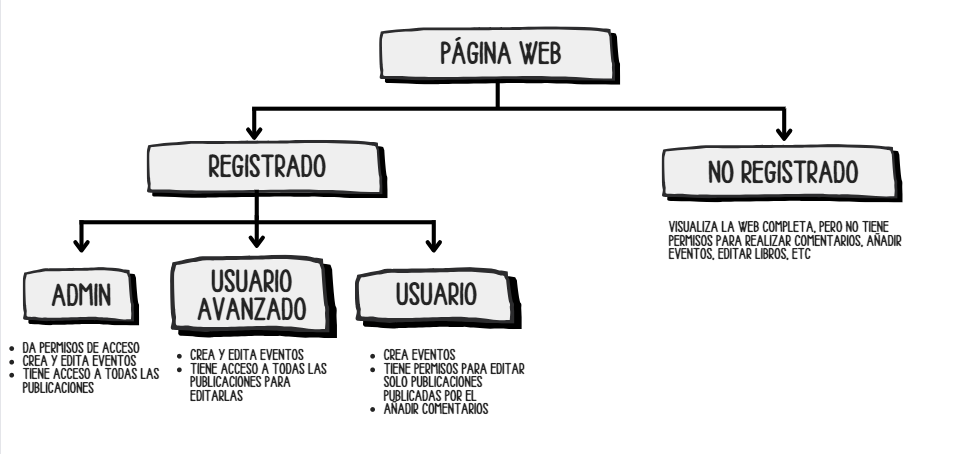
\includegraphics[width=0.7\textwidth]{img/esquema.png}
  \caption{Permisos de los Usuarios}
  \label{fig:arquitectura}
\end{figure}

La Figura (ver Figura~\ref{fig:arquitectura}) muestra un esquema general de la estructura de la página web. Esta página es accesible tanto para usuarios registrados 
como para visitantes, aunque la principal distinción entre estos dos roles radica en los privilegios que poseen.

Como visitante, se tiene acceso a la vista pública de la página, permitiendo visualizar el contenido ya publicado. No obstante, la interacción 
es limitada, ya que los visitantes no pueden comentar, subir nuevo contenido o interactuar con las publicaciones existentes.

Por otro lado, los usuarios registrados disfrutan de permisos adicionales que les permiten una interactuación amplia con la página. Además de ver el 
contenido, pueden participar activamente a través de comentarios, subir nuevo contenido y interactuar con las publicaciones existentes.

Este diseño permite a los visitantes explorar la web y, al mismo tiempo, incita a un mayor compromiso a través del registro, permitiendo así aprovechar 
todas las funciones que ofrece la plataforma.

\subsection{Vista de Usuario - No Registrado}
\label{sec:vista_usuarios_no_registrado}

En esta sección se detallan las diferentes páginas y archivos relacionados con la experiencia del usuario no registrado en la plataforma:
\begin{figure}
  \centering
  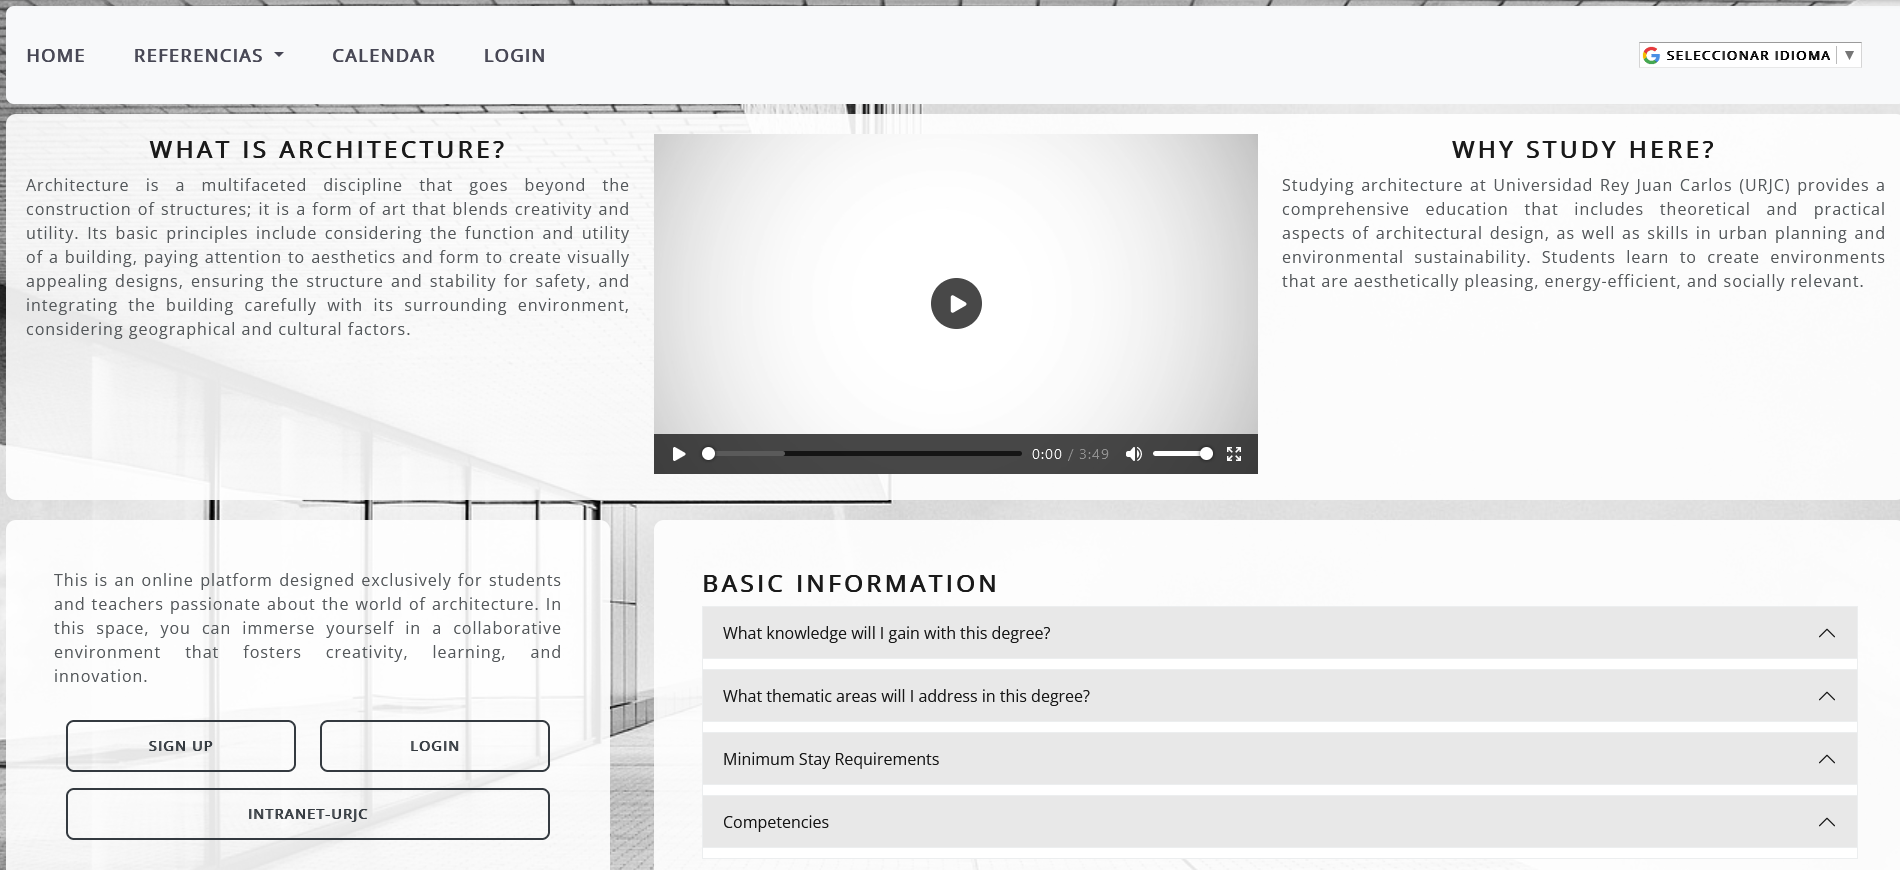
\includegraphics[width=0.6\textwidth]{img/sitio1.png}
  
\includegraphics[width=0.6\textwidth]{img/sitiopie.png}
  \caption{Vista de página principal}
  \label{fig:sitioindex}
\end{figure}
\begin{figure}
  \centering
  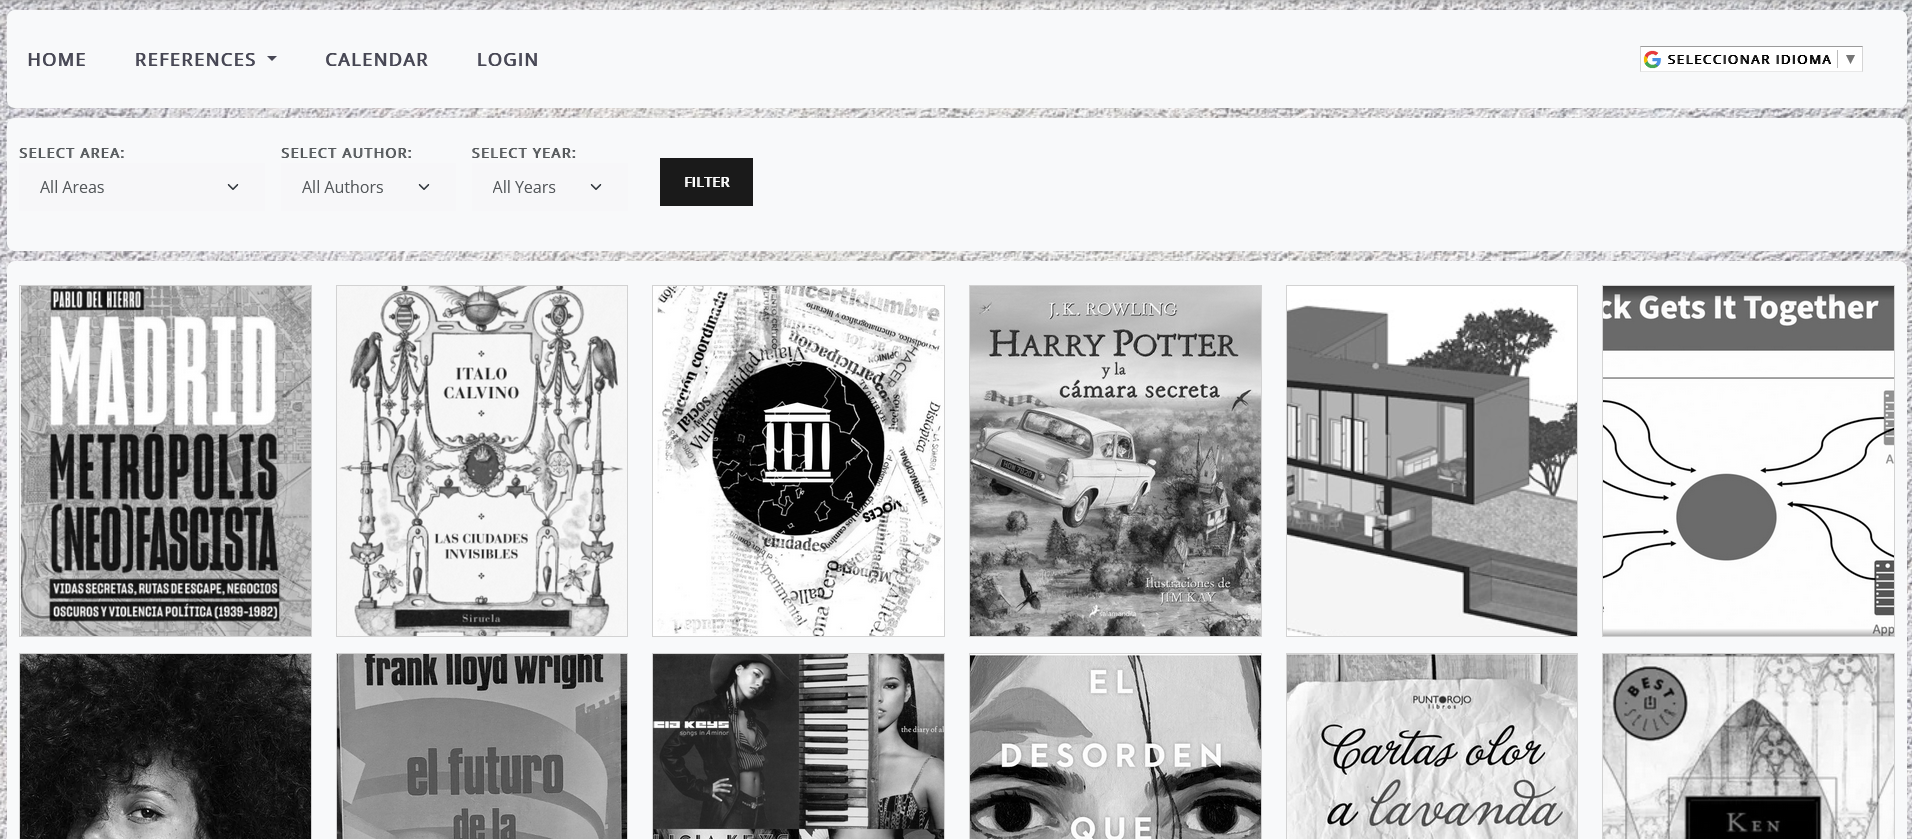
\includegraphics[width=0.6\textwidth]{img/booksitio.png}
  \caption{Vista de la página de libros}
  \label{fig:sitiobooks}
\end{figure}
\begin{figure}
  \centering
  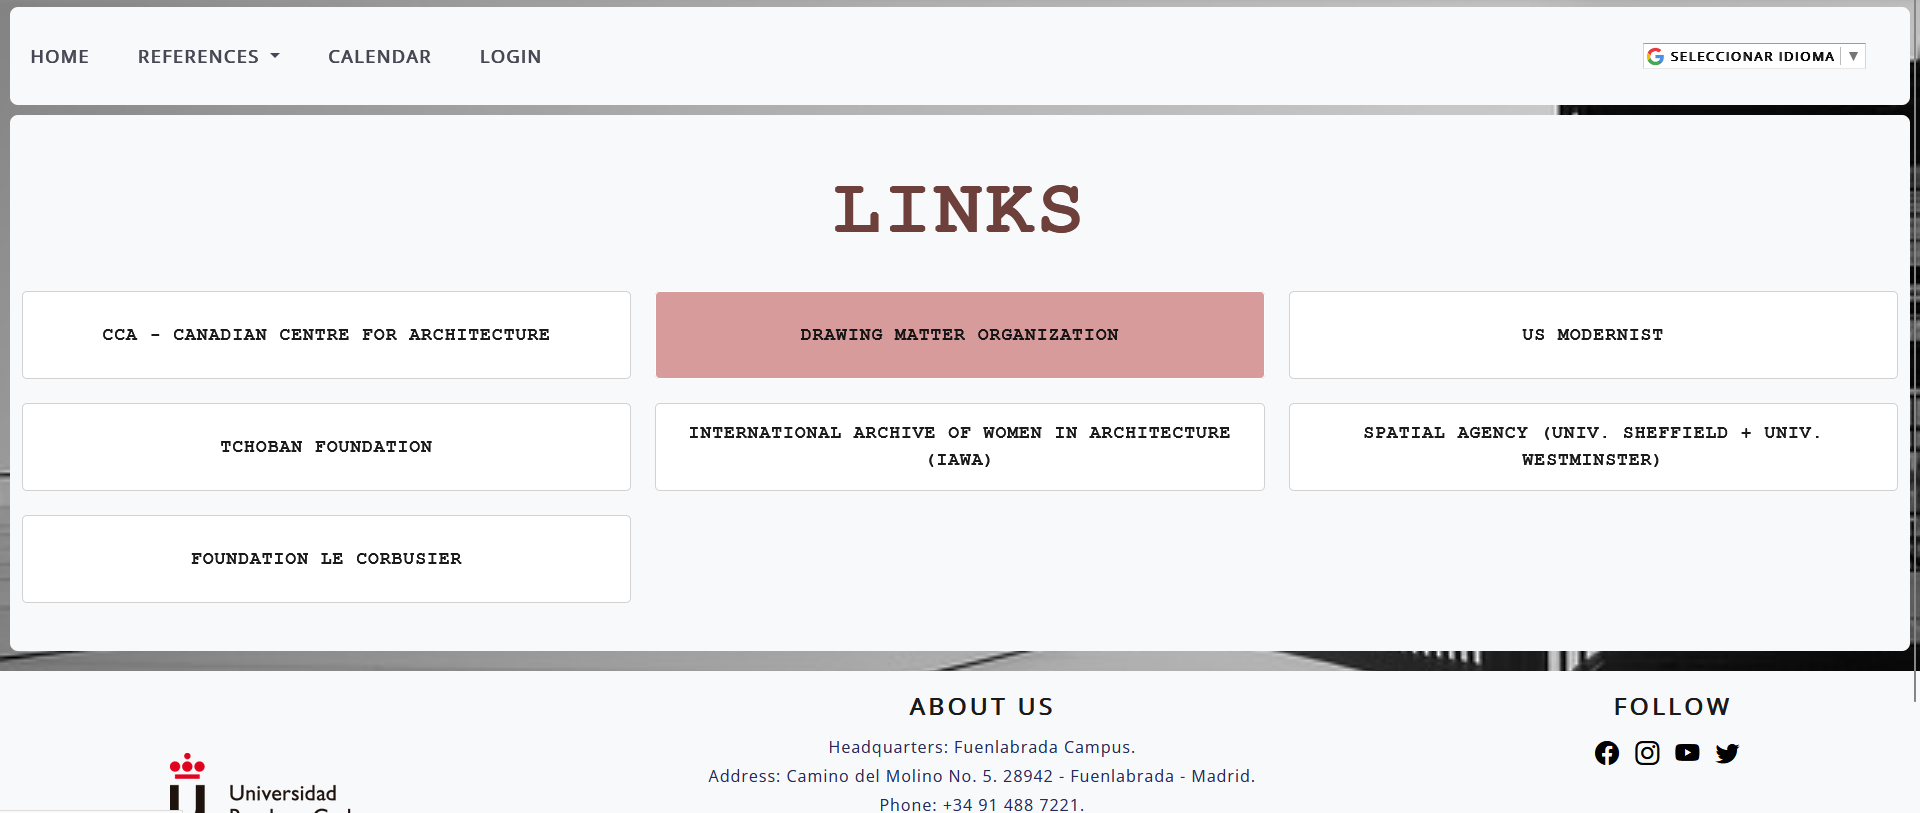
\includegraphics[width=0.6\textwidth]{img/linksitio.png}
  \caption{Vista de la página de links}
  \label{fig:sitiolinks}
\end{figure}

\begin{figure}
  \centering
  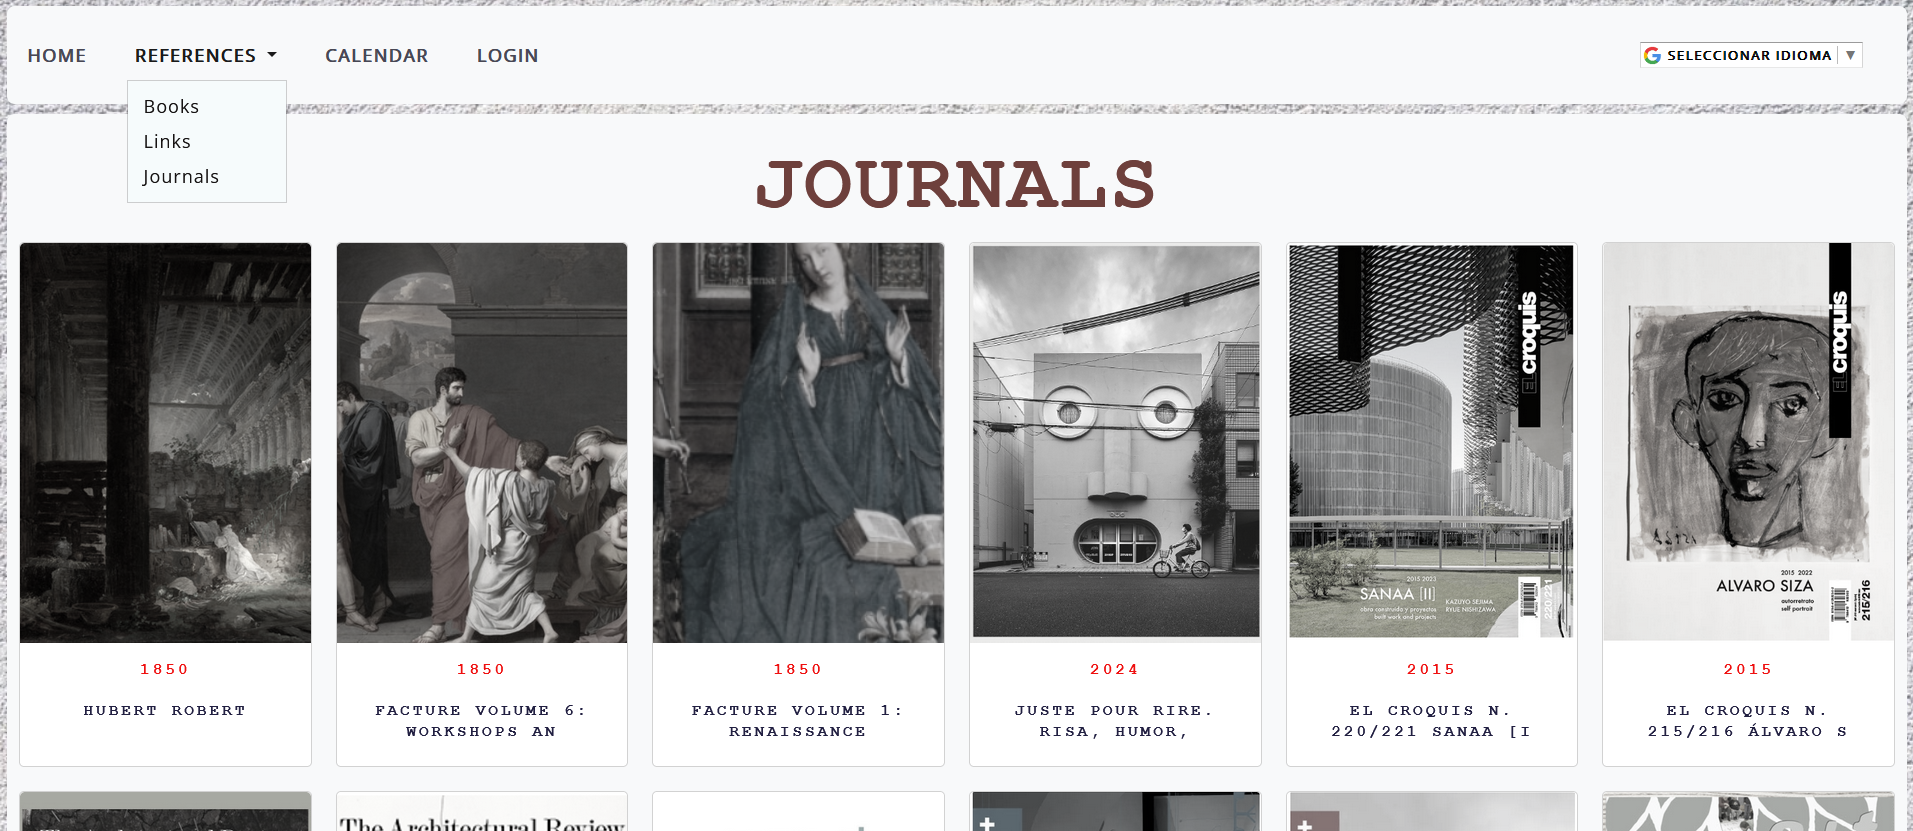
\includegraphics[width=0.6\textwidth]{img/revistassitio.png}
  \caption{Vista de la página de revistas}
  \label{fig:sitiojournals}
\end{figure}

\begin{figure}
  \centering
  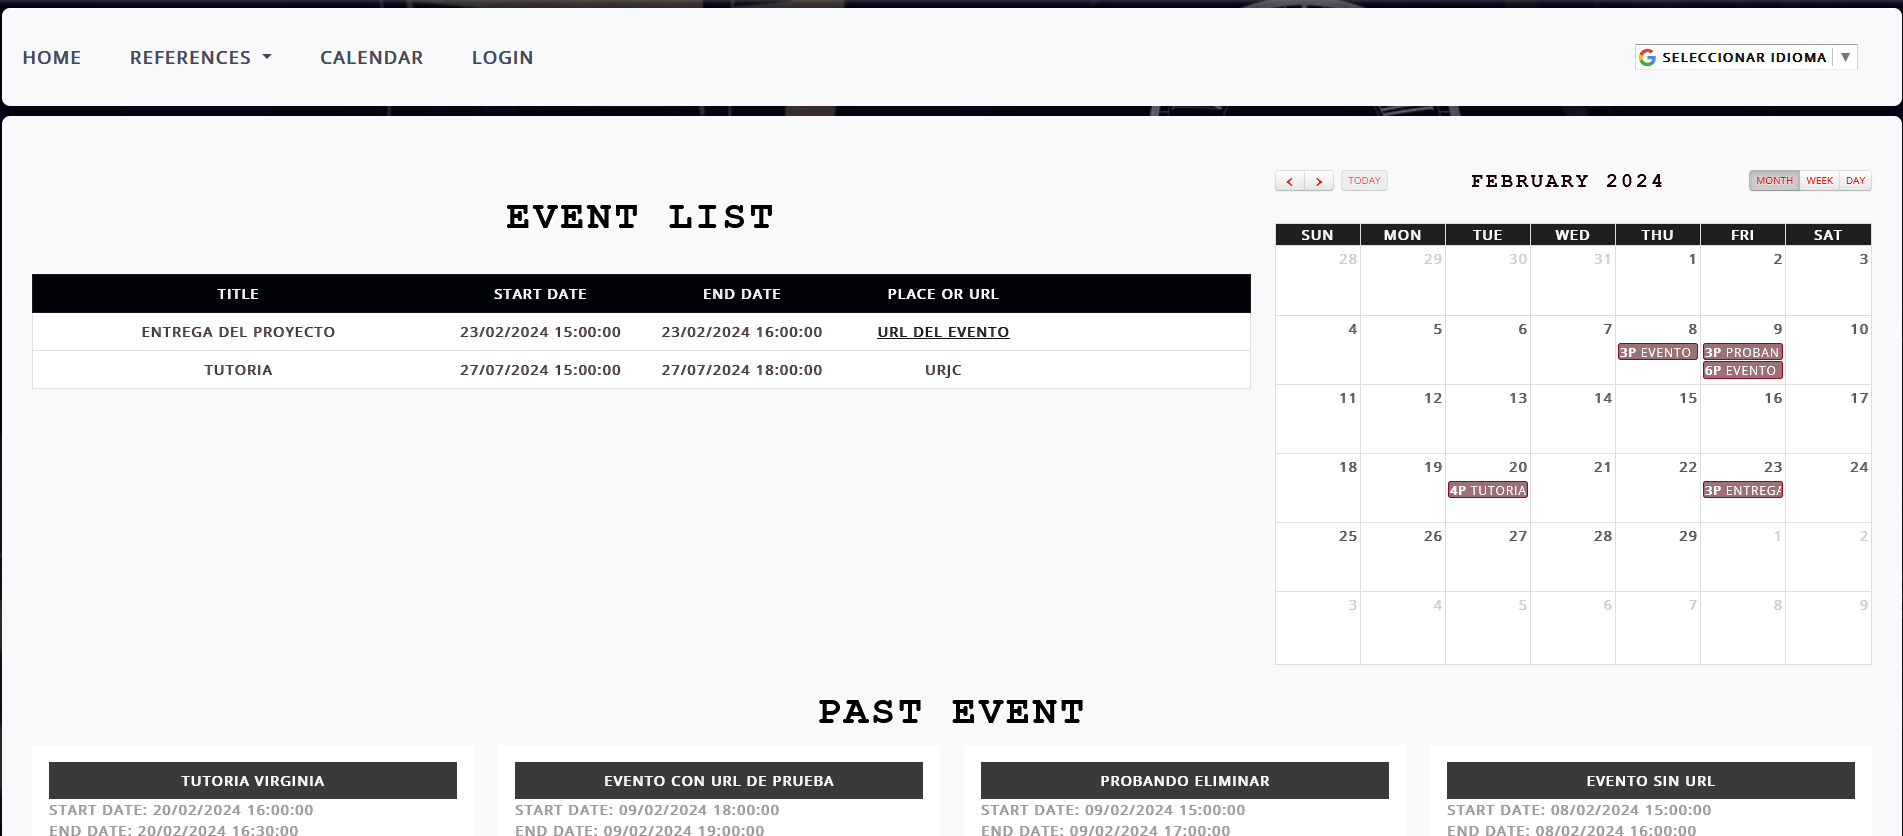
\includegraphics[width=0.6\textwidth]{img/calendarsitio.png}
  \caption{Vista de la página de calendario}
  \label{fig:sitiocalendar}
\end{figure}

\begin{itemize}
  \item \texttt{sitio/top\_of\_page.html}: Este archivo contiene la barra de navegación principal de la aplicación, que proporciona enlaces a diversas páginas y funcionalidades del sitio web.
  \item \texttt{sitio/index.html}: Se trata de la página de inicio de la plataforma (ver Figura~\ref{fig:sitioindex}), donde los usuarios pueden comenzar su navegación.
  \item \texttt{sitio/books.html}: Esta página muestra la estructura y propiedades de la sección de libros (ver Figura~\ref{fig:sitiobooks}), donde los usuarios pueden explorar los libros disponibles en la plataforma y obtener más detalles sobre ellos.
  \item \texttt{sitio/calendar.html}: Aquí se presenta el calendario (ver Figura~\ref{fig:sitiocalendar}), mostrando eventos presentes y futuros relevantes para los usuarios.
  \item \texttt{sitio/filterForm.html}: Ofrece a los usuarios la posibilidad de filtrar el contenido según ciertos criterios establecidos.
  \item \texttt{sitio/journals.html}: Define la estructura y características de la sección de revistas~\ref{fig:sitiojournals}, donde se muestran las revistas disponibles en la plataforma.
  \item \texttt{sitio/links.html}: En esta página se muestran los enlaces (ver Figura~\ref{fig:sitiolinks}) disponibles para los usuarios.
  \item \texttt{sitio/footer.html}: Es el pie de página que se muestra en todas las páginas de la plataforma, proporcionando información adicional y enlaces útiles.
  \item \texttt{base.html}: Define la apariencia general común a todas las páginas, permitiendo que cada página hija llene bloques específicos con su título y contenido.
  \item \texttt{detalle\_libro.html}: Presenta detalles específicos de un libro, permitiendo a los usuarios agregar comentarios sobre el libro y al administrador eliminar comentarios si es necesario.
  \item \texttt{error.html}: Proporciona una interfaz amigable para mostrar mensajes de error a los usuarios en caso de que ocurra algún problema, ofreciéndoles la opción de volver a la página anterior.
\end{itemize}

Estos archivos constituyen los elementos fundamentales que componen la experiencia de usuario para aquellos que aún no se han registrado en la plataforma.

\subsection{Vista de Usuario - Registrado}
\label{sec:vista_usuarios_registrado}
En esta sección se detallan las diferentes páginas y archivos relacionados con la experiencia de usuarios registrados en la plataforma:

\begin{itemize}
  \item \texttt{admin/top\_of\_page.html}: Este archivo define la barra de navegación en la sección de administración del sitio web. Incluye enlaces para las páginas de inicio, libros, links, revistas, calendario y cierre de sesión. Además, muestra un enlace adicional para la página de permisos si la {'id\_rol'} del usuario en sesión es igual a 1. También proporciona un traductor de Google para cambiar el idioma del contenido.
  \item \texttt{admin/calendar.html}: En esta página se presenta el calendario (ver Figura~\ref{fig:admincal}), que permite la creación, edición y eliminación de eventos pasados, presentes y futuros, dependiendo del rol del usuario identificado por su id\_rol.
  \item \texttt{admin/index.html}: Esta es la vista de la página de inicio del administrador en el sitio web. Ofrece un mensaje de bienvenida, información sobre la comunidad de arquitectura y enumera las expectativas para los miembros de la comunidad.
  \item \texttt{admin/books.html}: Aquí se encuentra una interfaz para cargar libros al sitio desde la sección de administración. Incluye un formulario con campos para ingresar detalles como el título del libro, imagen de portada, nombre y apellido del autor, URL, descripción, video, archivo PDF... Además, permite seleccionar el año y el área. También muestra los documentos existentes en la plataforma.
  \item \texttt{admin/documents.html}: Esta vista muestra una tabla para gestionar los libros cargados en la página de administración del sitio web. Proporciona una lista de todos los libros mostrando su título y autor. Para cada libro, se ofrecen acciones para eliminar, visualizar y editar los detalles de los libros.
  \item \texttt{admin/editar\_libro.html}: Proporciona una interfaz para editar los detalles de un libro {(Previamente cargados de la base de datos)}. Incluye un formulario con campos para el título, imagen de portada, URL, año de publicación, área de estudio, nombre y apellido del autor, descripción, y opción de agregar o eliminar archivos multimedia como vídeo, archivo PDF o imagen secundaria.
  \item \texttt{admin/journals.html}: Ofrece una interfaz para gestionar revistas en la sección de administración. Incluye un formulario para añadir una nueva revista con campos para título, año, enlace y portada. También muestra una tabla con todas las revistas existentes, proporcionando opciones para eliminarlas.
  \item \texttt{admin/links.html}: Proporciona una interfaz para administrar enlaces en la sección de administración del sitio web. Permite agregar nuevos enlaces a través de un formulario que solicita título y URL, y muestra una tabla con todos los enlaces existentes, con opciones para eliminarlos.
  \item \texttt{admin/login.html}: Es la interfaz de inicio de sesión (ver Figura~\ref{fig:adminacceso}) para el área de administración del sitio web. Permite a los usuarios craer una cuentas, iniciar sesión ingresando su nombre de usuario y contraseña tambien dipone de un enlace para recuperar la contraseña en caso de olvido.
  \item \texttt{admin/olvide\_contrasena.html}: Proporciona una interfaz para que los usuarios recuperen sus contraseñas en caso de olvido. Solicita al usuario ingresar su dirección de correo electrónico y, al enviar el formulario, se envía una solicitud para restablecer la contraseña a esa dirección de correo electrónico.
  \item \texttt{admin/restablecer\_contrasena.html}: Permite a los usuarios restablecer sus contraseñas después de solicitar un restablecimiento. Los usuarios pueden ingresar su nueva contraseña en un formulario y, al enviarlo, la aplicación tomará esa nueva contraseña y la establecerá como la contraseña actual del usuario.
  \item \texttt{admin/registro.html}: Proporciona un formulario de registro de usuario. Permite a los nuevos usuarios crear un perfil en el sitio web proporcionando un nombre de usuario, contraseña y dirección de correo electrónico. Después de la presentación exitosa, se envía un correo electrónico de confirmación a la dirección de correo electrónico proporcionada.
  \item \texttt{admin/permisos.html}: Ofrece una interfaz para gestionar usuarios y sus permisos en el dashboard de administración del sitio web. Muestra en una tabla el nombre de usuario, correo electrónico y rol de cada usuario registrado. El administrador puede cambiar el rol de un usuario y eliminar usuarios. También muestra el estatus de aprobación para el acceso del usuario y permite al administrador aceptar o rechazar la solicitud de acceso.
\end{itemize}

Estos archivos constituyen los elementos fundamentales que componen la experiencia de usuarios que se han registrado o que están por registrarse en la plataforma.
\begin{figure}
  \centering
  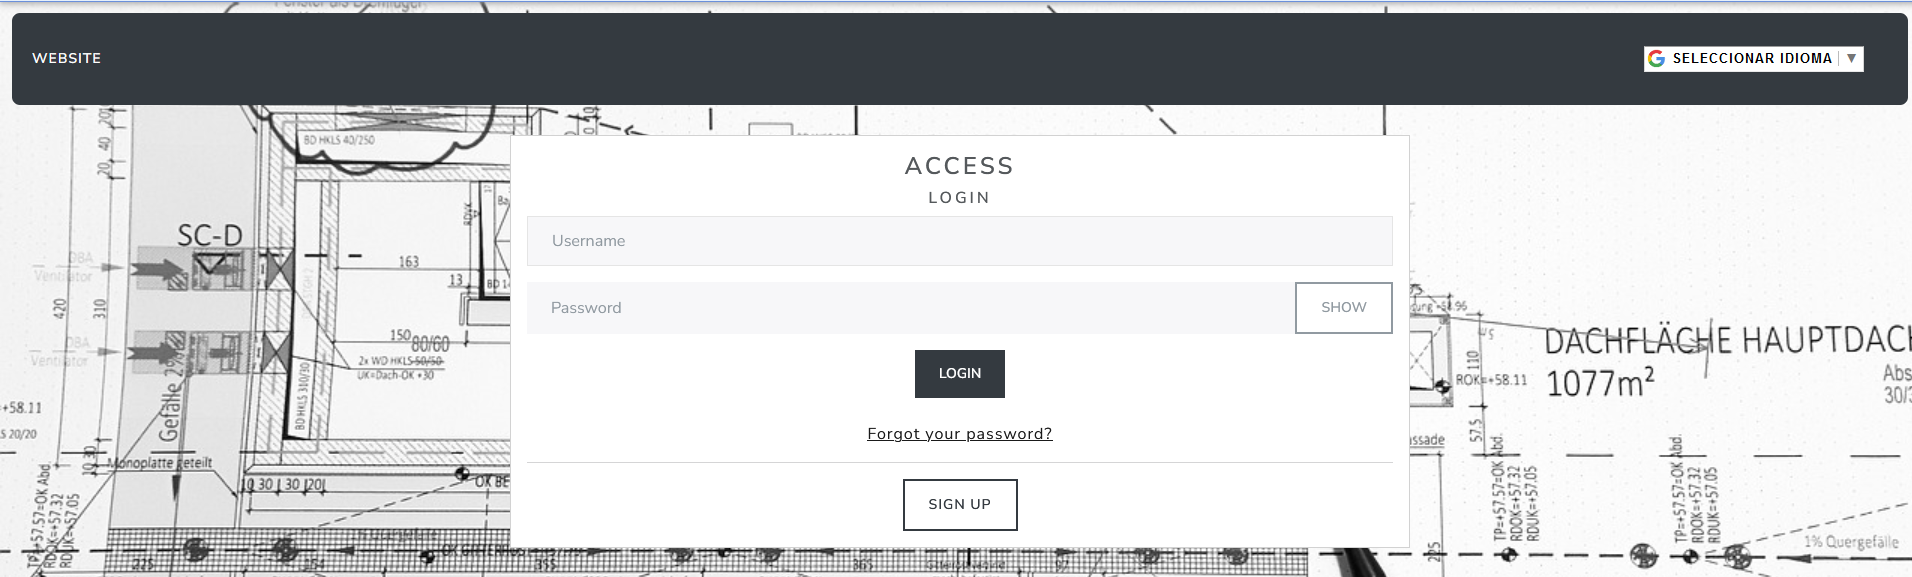
\includegraphics[width=0.6\textwidth]{img/acceso.png}
  \caption{Acceso de a la plataforma}
  \label{fig:adminacceso}
\end{figure}
\begin{figure}
  \centering
  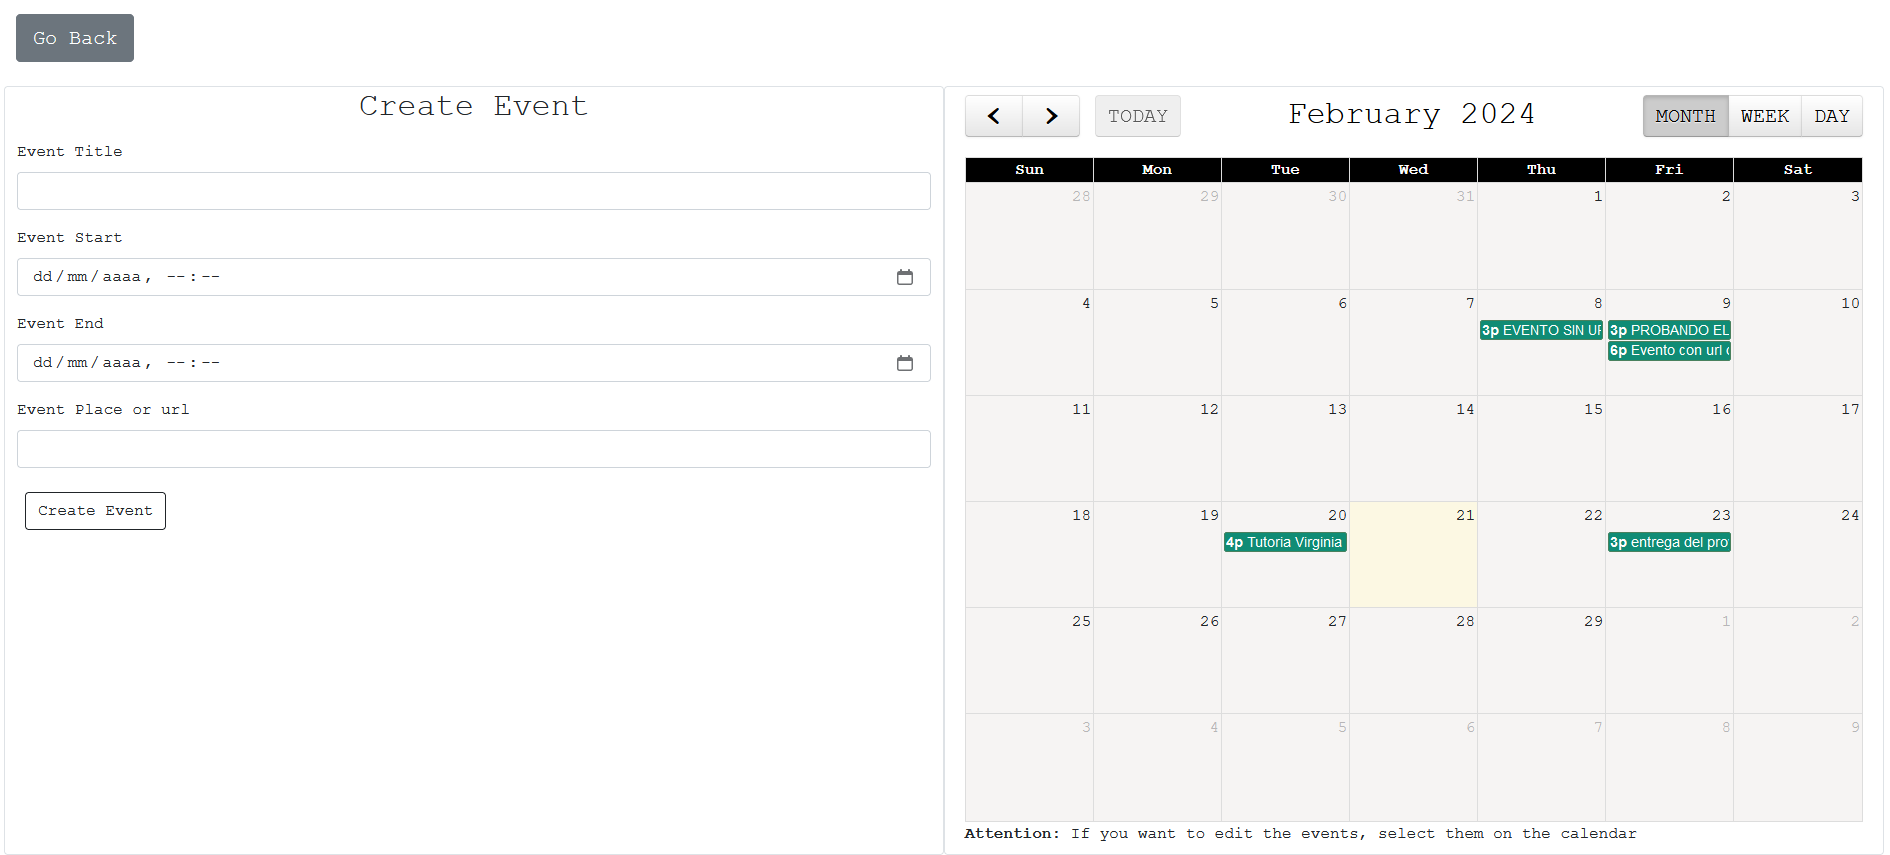
\includegraphics[width=0.6\textwidth]{img/calendarioadmin.png}
  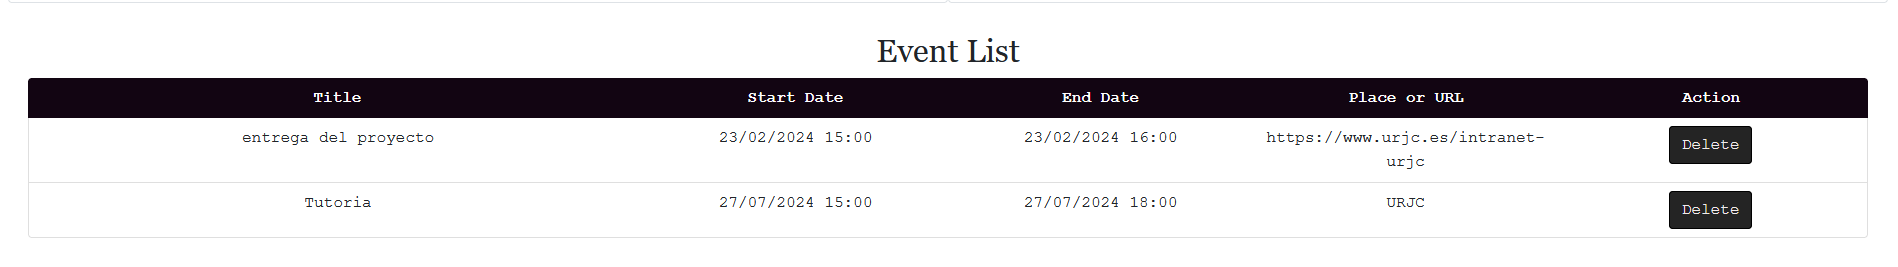
\includegraphics[width=0.6\textwidth]{img/calendarioadmin2.png}
  \caption{Calendario desde admin}
  \label{fig:admincal}
\end{figure}

%%%%%%%%%%%%%%%%%%%%%%%%%%%%%%%%%%%%%%%%%%%%%%%%%%%%%%%%%%%%%%%%%%%%%%%%%%%%%%%%
%%%%%%%%%%%%%%%%%%%%%%%%%%%%%%%%%%%%%%%%%%%%%%%%%%%%%%%%%%%%%%%%%%%%%%%%%%%%%%%%
% EXPERIMENTOS Y VALIDACIÓN %
%%%%%%%%%%%%%%%%%%%%%%%%%%%%%%%%%%%%%%%%%%%%%%%%%%%%%%%%%%%%%%%%%%%%%%%%%%%%%%%%

\cleardoublepage
\chapter{Experimentos y validación}
\label{chap:experimentos}

En este capítulo se explicaran las diferentes pruebas que se fueron realizando durante el desarrollo de este proyectos.

\section{Pruebas con la aplicación}
\label{sec:pruebas}

A lo largo del desarrollo del proyecto, se llevaron a cabo pruebas continuas para evaluar y garantizar el correcto funcionamiento del 
sistema en todas sus etapas. Estas pruebas se realizaron de manera periódica y sistemática, abarcando diferentes aspectos del proyecto, 
desde la funcionalidad básica hasta características más específicas. El objetivo principal de estas pruebas fue detectar y corregir 
cualquier problema o inconveniente lo antes posible, asegurando así la calidad y la fiabilidad del producto final. Este enfoque 
contribuyó significativamente a la mejora continua del proyecto y a la entrega de un proyecto final de alta calidad.
\subsection{Pruebas Funcionales}
\label{sec:funcionalidad}
Nuestro objetivo es garantizar el funcionamiento óptimo de todas las rutas y funciones del sistema. Para lograr esto, realizamos 
una exhaustiva validación de formularios y enlaces, asegurándonos de que cada elemento de la interfaz de usuario funcione de manera 
correcta y coherente. Esta revisión minuciosa nos permite identificar cualquier posible inconveniente o error en la navegación y la 
interacción del usuario (ver Figura~\ref{fig:errorse}), asegurando así una experiencia fluida y satisfactoria para todos los usuarios que ocupen la página web.

\begin{figure}
  \centering
  
\includegraphics[width=0.6\textwidth]{img/error.png}
  \caption{Mensajes de error}
  \label{fig:errorse}
\end{figure}

\subsection{Validación de Formularios}
\label{sec:validacion}
Se llevaron a cabo una serie de pruebas exhaustivas para asegurar el correcto funcionamiento de las validaciones del formulario 
en diversas acciones, como la subida, publicación o edición de un libro o evento, así como en el registro de usuarios.
Durante este proceso, nos aseguramos de que cada aspecto del formulario se comporte como se espera(ver Figura~\ref{fig:form}). En caso de que se introduzcan 
datos incorrectos, verificamos que se muestren los mensajes de error correspondientes, proporcionando así una retroalimentación 
clara al usuario. Además, nos aseguramos de que cada elemento del formulario cumpla adecuadamente su función asignada, garantizando 
una experiencia fluida y sin contratiempos para el usuario final.
\begin{figure}
  \centering
  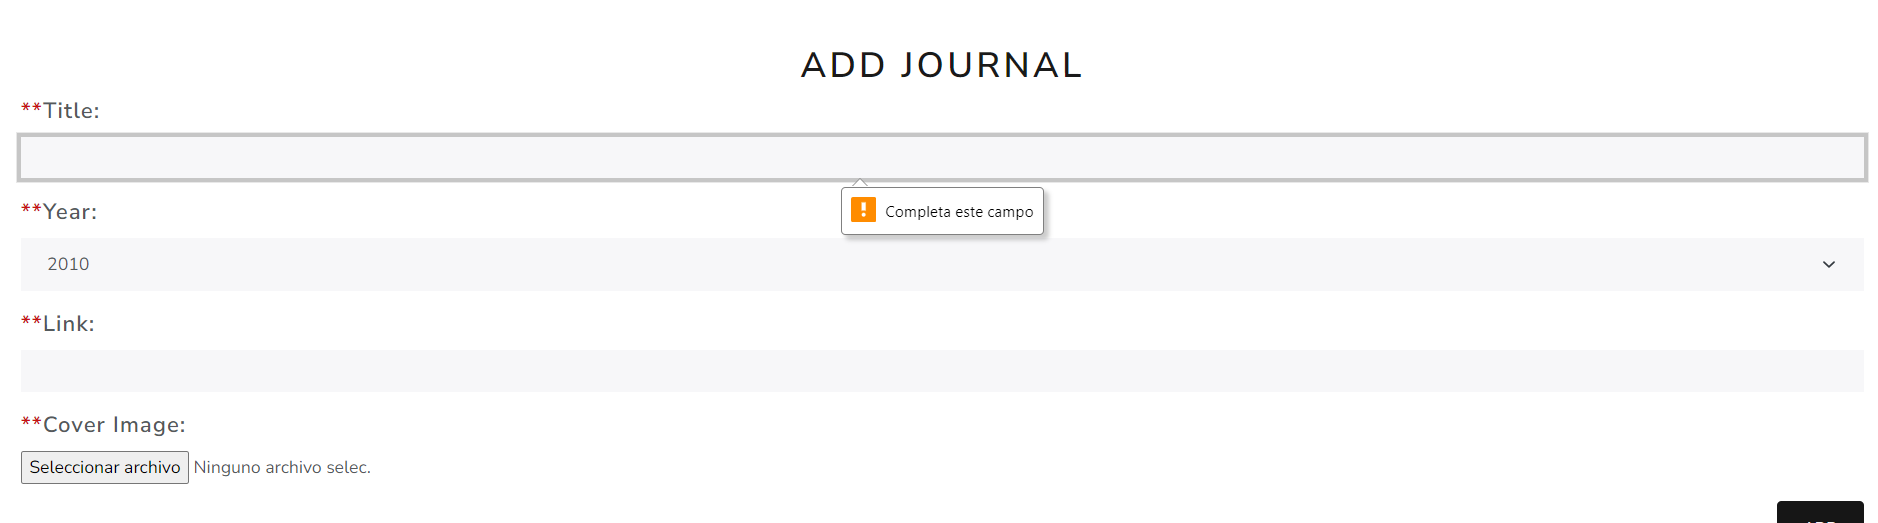
\includegraphics[width=0.6\textwidth]{img/formulario.png}
  \caption{Alerta: Faltan datos en el formulario}
  \label{fig:form}
\end{figure}
\subsection{Pruebas de Compatibilidad e Interfaz de Usuario (UI)}
\label{sec:compatibilidad}
Nuestra prioridad es garantizar la coherencia y la funcionalidad del sistema en una amplia variedad de entornos. Realizamos exhaustivas 
pruebas para verificar que el sistema se comporte de manera uniforme en diferentes navegadores y dispositivos (ver Figura~\ref{fig:movil}). 
Nos esforzamos por asegurar que cada página mantenga su apariencia y funcionalidad óptimas, sin importar la resolución de pantalla utilizada. De esta 
manera, nos aseguramos de proporcionar una experiencia de usuario consistente y satisfactoria en todas las circunstancias.
\begin{figure}
  \centering
  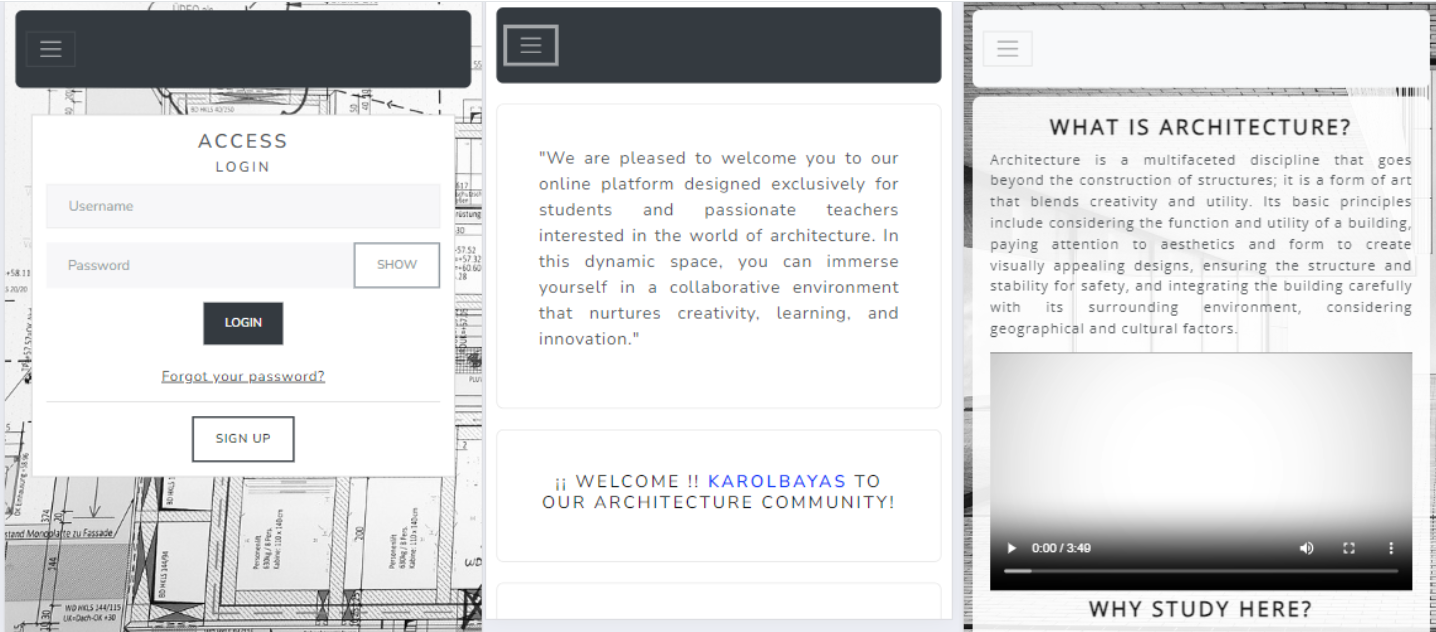
\includegraphics[width=0.6\textwidth]{img/vistamovil.png}
  \caption{Vista desde un dispositivo movil}
  \label{fig:movil}
\end{figure}

\subsection{Pruebas de la Base de Datos}
\label{sec:base_datos}
Se lleva a cabo una exhaustiva verificación para asegurar el correcto funcionamiento de las consultas a la base de datos 
(ver Figura~\ref{fig:db}). Se realizan pruebas detalladas para garantizar la precisión y la eficacia de cada interacción 
con la base de datos, asegurando así la integridad y la fiabilidad de los datos recuperados y procesados.

\begin{figure}
  \centering
  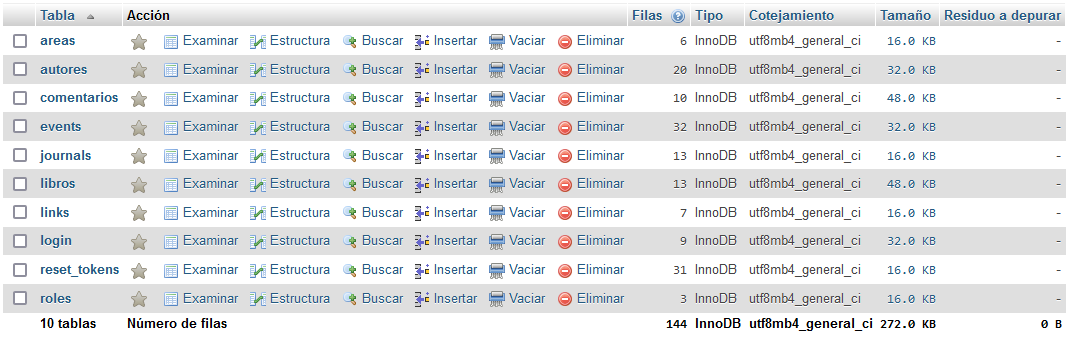
\includegraphics[width=0.6\textwidth]{img/db.png}
  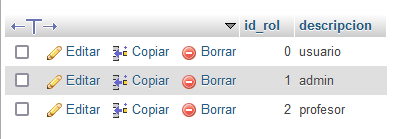
\includegraphics[width=0.6\textwidth]{img/roldb.png}
  \caption{Base de datos}
  \label{fig:db}
\end{figure}


%%%%%%%%%%%%%%%%%%%%%%%%%%%%%%%%%%%%%%%%%%%%%%%%%%%%%%%%%%%%%%%%%%%%%%%%%%%%%%%%
%%%%%%%%%%%%%%%%%%%%%%%%%%%%%%%%%%%%%%%%%%%%%%%%%%%%%%%%%%%%%%%%%%%%%%%%%%%%%%%%
% RESULTADOS %
%%%%%%%%%%%%%%%%%%%%%%%%%%%%%%%%%%%%%%%%%%%%%%%%%%%%%%%%%%%%%%%%%%%%%%%%%%%%%%%%

\cleardoublepage
\chapter{Resultados}
\label{chap:resultados}

En el capítulo de resultados, se realizaron diversas pruebas para evaluar las funcionalidades de la plataforma en varios aspectos. Se centraron en la 
capacidad de cargar y eliminar libros, enlaces, revistas y eventos, asegurando que cada operación se llevara a cabo de manera adecuada y sin contratiempos.

\section{Descripcion de las pruebas realizadas}
\label{sec:pruebas}
El capítulo de resultados presenta una serie de pruebas realizadas para evaluar diversas funcionalidades de la plataforma en diferentes aspectos. Aquí se detallan las 
pruebas realizadas y las conclusiones obtenidas:

\subsection{ Realizar Login o Registro de Usuarios}
\label{sec:login-registro}
Se evaluó la capacidad de la plataforma para manejar el inicio de sesión de los usuarios registrados y el registro de nuevos usuarios, además de realizar las siguientes comprobaciones adicionales:
  \begin{itemize}
    \item \textbf{Envío de correo de registro:} Se verificó que el correo electrónico de confirmación de registro se enviara correctamente a los nuevos usuarios 
    después de registrarse en la plataforma.(ver Figura~\ref{fig:registrook})
    \item \textbf{Validación de nombre de usuario único:} Se aseguró de que no pudiera existir más de un usuario con el mismo nombre de usuario. Esta validación 
    garantiza la unicidad de los nombres de usuario en la plataforma. (ver Figura~\ref{fig:usernameerror})
    \item \textbf{Acceso restringido hasta que se otorgue permiso:}  Se comprobó que los usuarios no pudieran acceder a la aplicación hasta que se les otorgara acceso. 
    Esto asegura que solo los usuarios autorizados puedan utilizar la plataforma una vez que se les haya dado permiso.(ver Figura~\ref{fig:waiting})
  \end{itemize}

  \begin{figure}
    \centering
    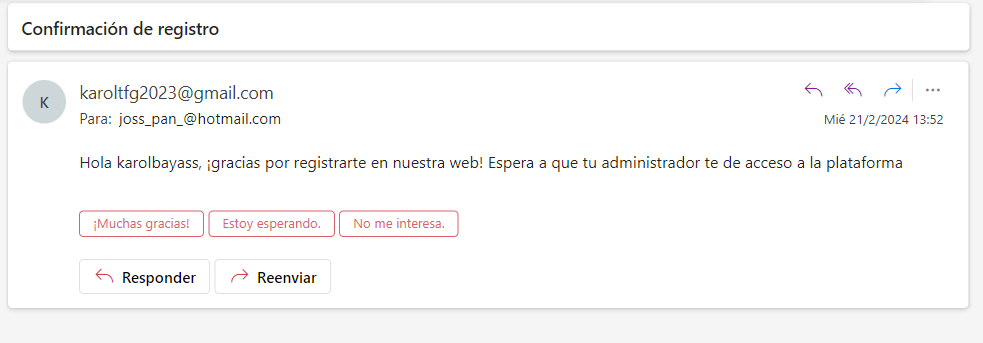
\includegraphics[width=0.5\textwidth]{img/correoresgistro.png}
    \caption{Correo de Registro Correcto}
    \label{fig:registrook}
  \end{figure}
  \begin{figure}
    \centering
    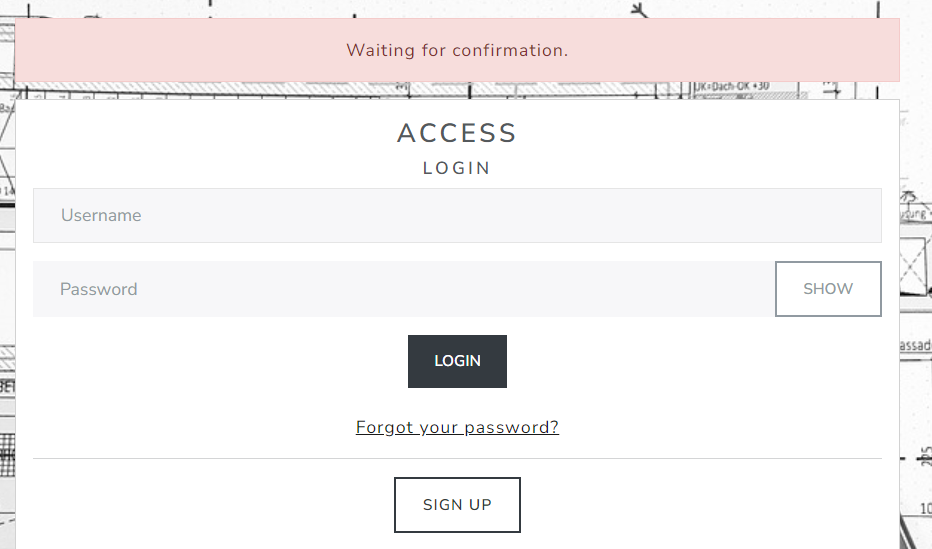
\includegraphics[width=0.5\textwidth]{img/confacceso.png}
    \caption{Mensaje: Esperando confirmación}
    \label{fig:waiting}
  \end{figure}

  \begin{figure}
    \centering
    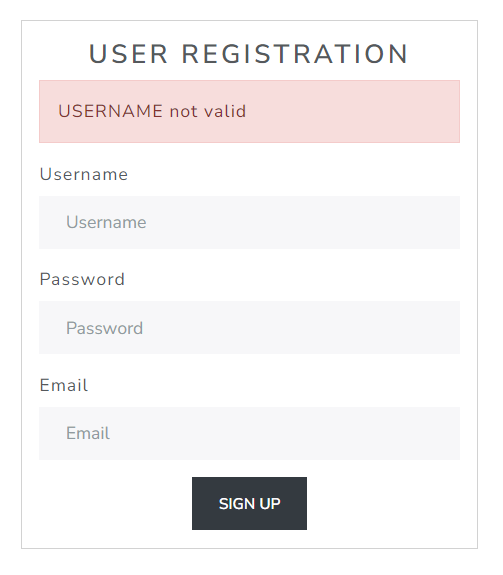
\includegraphics[width=0.7\textwidth]{img/username.png}
    \caption{Mensaje: Username not valid}
    \label{fig:usernameerror}
  \end{figure}

\subsection{Recuperación de Contraseña}
\label{sec:recuperacion-contraseña}
Durante esta prueba, se evaluó la funcionalidad de recuperación de contraseña de la plataforma (ver Figura~\ref{fig:contrasenarest}). Se verificó que los usuarios 
pudieran restablecer su contraseña en caso de olvidarla o necesitar cambiarla por motivos de seguridad. El proceso de recuperación de contraseña debe ser intuitivo 
y seguro, garantizando que solo el usuario legítimo pueda restablecer su contraseña. Para ello, se implementó un sistema que envía un correo electrónico con un enlace 
único y seguro que permite al usuario restablecer su contraseña. Se evaluaron aspectos como la recepción del correo electrónico de restablecimiento de contraseña, 
la seguridad de los enlaces de restablecimiento enviados por correo electrónico y la facilidad de uso del proceso en general. Esta funcionalidad es fundamental 
para la seguridad y la experiencia del usuario en la plataforma.
\begin{figure}
  \centering
  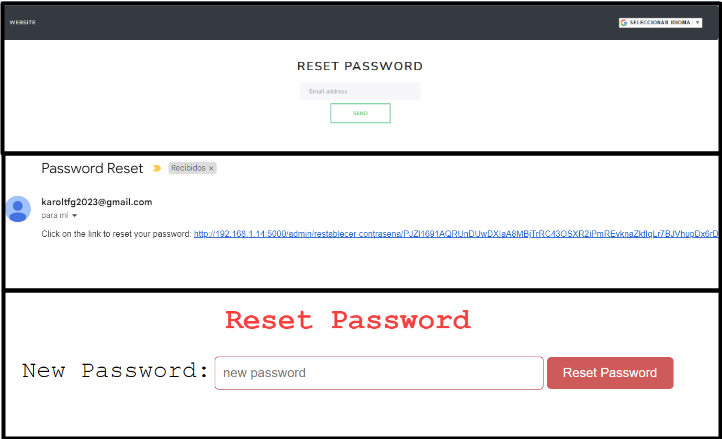
\includegraphics[width=0.7\textwidth]{img/password.png}
  \caption{Restablecer contraseña}
  \label{fig:contrasenarest}
\end{figure}

\subsection{Gestión de Eventos: Añadir, Eliminar y Editar}
\label{sec:add-delete-edit-events}

Durante esta evaluación, pusimos a prueba la capacidad de la plataforma para administrar eventos (ver Figura~\ref{fig:calendarioadmin}). Nos aseguramos de que los 
usuarios con los permisos adecuados pudieran realizar tres funciones clave: añadir, eliminar y editar eventos, de manera eficiente y sin inconvenientes. 

Para comenzar, nos centramos en el proceso de añadir un nuevo evento, asegurándonos de que fuera intuitivo y claro para los usuarios. Queríamos que pudieran 
ingresar fácilmente toda la información necesaria, como el título del evento, la fecha y la ubicación, sin complicaciones innecesarias.

Además, verificamos que los usuarios autorizados pudieran eliminar eventos existentes cuando fuera necesario. Esta función es vital para mantener actualizada 
la plataforma y garantizar que solo se muestren eventos relevantes.

La funcionalidad de edición de eventos también fue sometida a pruebas. Nos aseguramos de que los usuarios pudieran modificar con precisión los detalles de 
un evento, como el título, la fecha y la ubicación, sin cometer errores. Validamos cuidadosamente los datos introducidos durante la edición, evitando fechas 
incoherentes o información incorrecta.

En resumen, esta evaluación demostró que la plataforma puede gestionar eficazmente todo el ciclo de vida de los eventos, desde su creación inicial hasta 
cualquier modificación o eliminación necesaria, proporcionando una experiencia fluida y sin complicaciones para todos los usuarios.

\begin{figure}
  \centering
  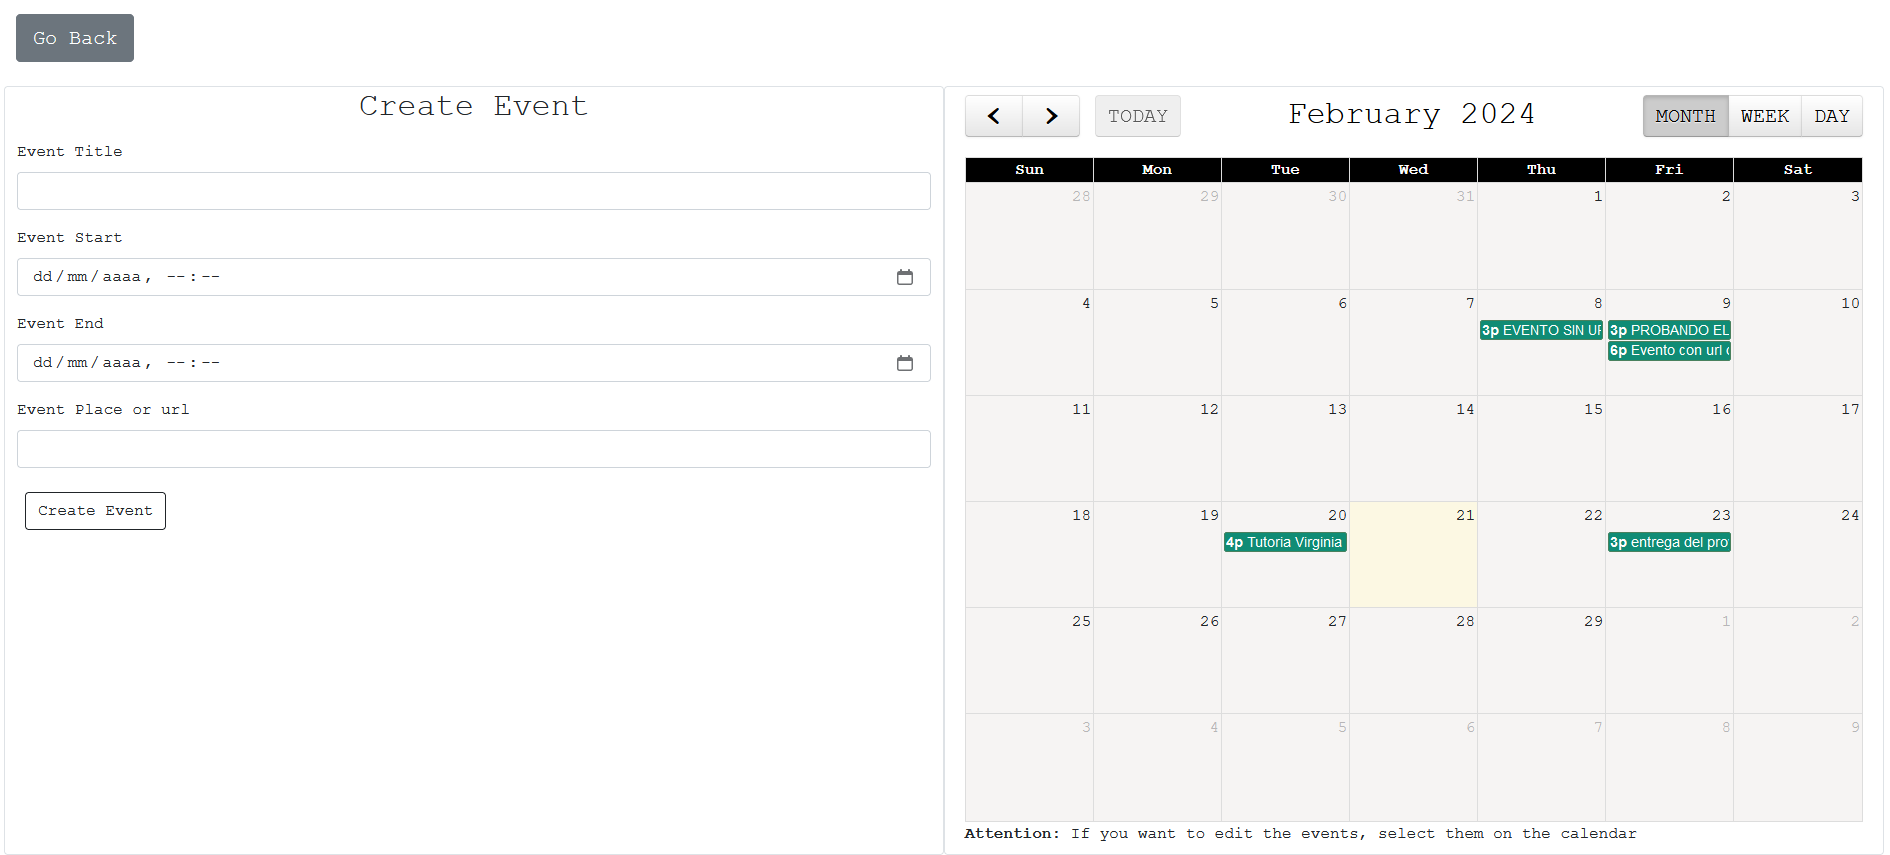
\includegraphics[width=0.7\textwidth]{img/calendarioadmin.png}
  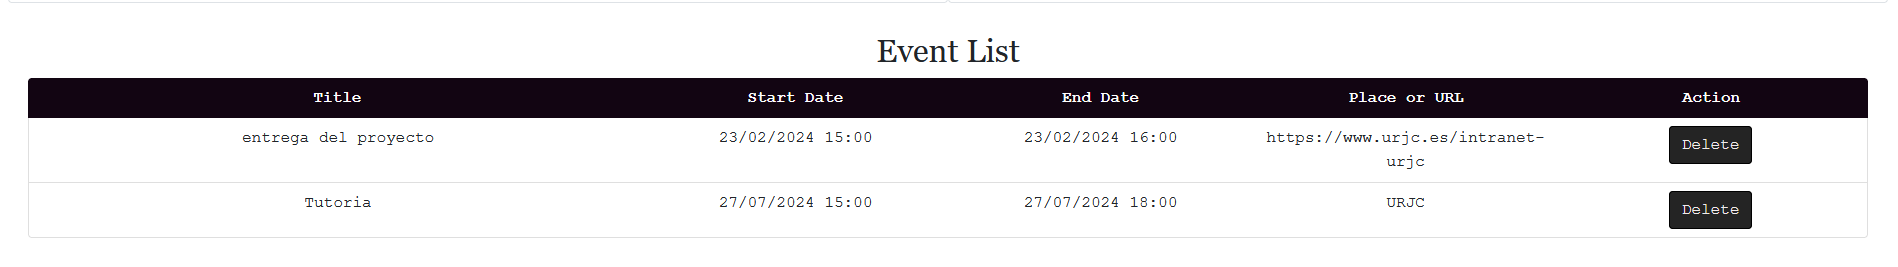
\includegraphics[width=0.7\textwidth]{img/calendarioadmin2.png}
  \caption{Calendario desde Administrador}
  \label{fig:calendarioadmin}
\end{figure}

\subsection{Gestión de Enlaces y Revistas: Añadir y Eliminar}
\label{sec:add-delete-links-magazines}

En esta fase de evaluación, nos concentramos en la capacidad de la plataforma para administrar enlaces y revistas, centrándonos en las operaciones de 
añadir y eliminar. (ver Figura~\ref{fig:journadmin})

Primero, nos aseguramos de que los usuarios autorizados pudieran añadir nuevos enlaces o revistas de manera sencilla y eficiente. Nos preocupamos por 
que el proceso de añadir fuera claro y directo, permitiendo a los usuarios ingresar la información necesaria de manera fluida, como el título, la URL 
(en el caso de los enlaces) o los detalles de la revista.

Seguidamente, evaluamos la función de eliminación para garantizar que los usuarios pudieran eliminar enlaces o revistas existentes según fuera necesario. 
Esta capacidad es crucial para mantener actualizada la plataforma y garantizar que solo se muestren recursos relevantes y válidos.

En resumen, durante esta evaluación, confirmamos que la plataforma puede gestionar de manera efectiva la adición y eliminación de enlaces y revistas, 
proporcionando a los usuarios una experiencia sin complicaciones y garantizando la integridad de los recursos mostrados.

\begin{figure}
  \centering
  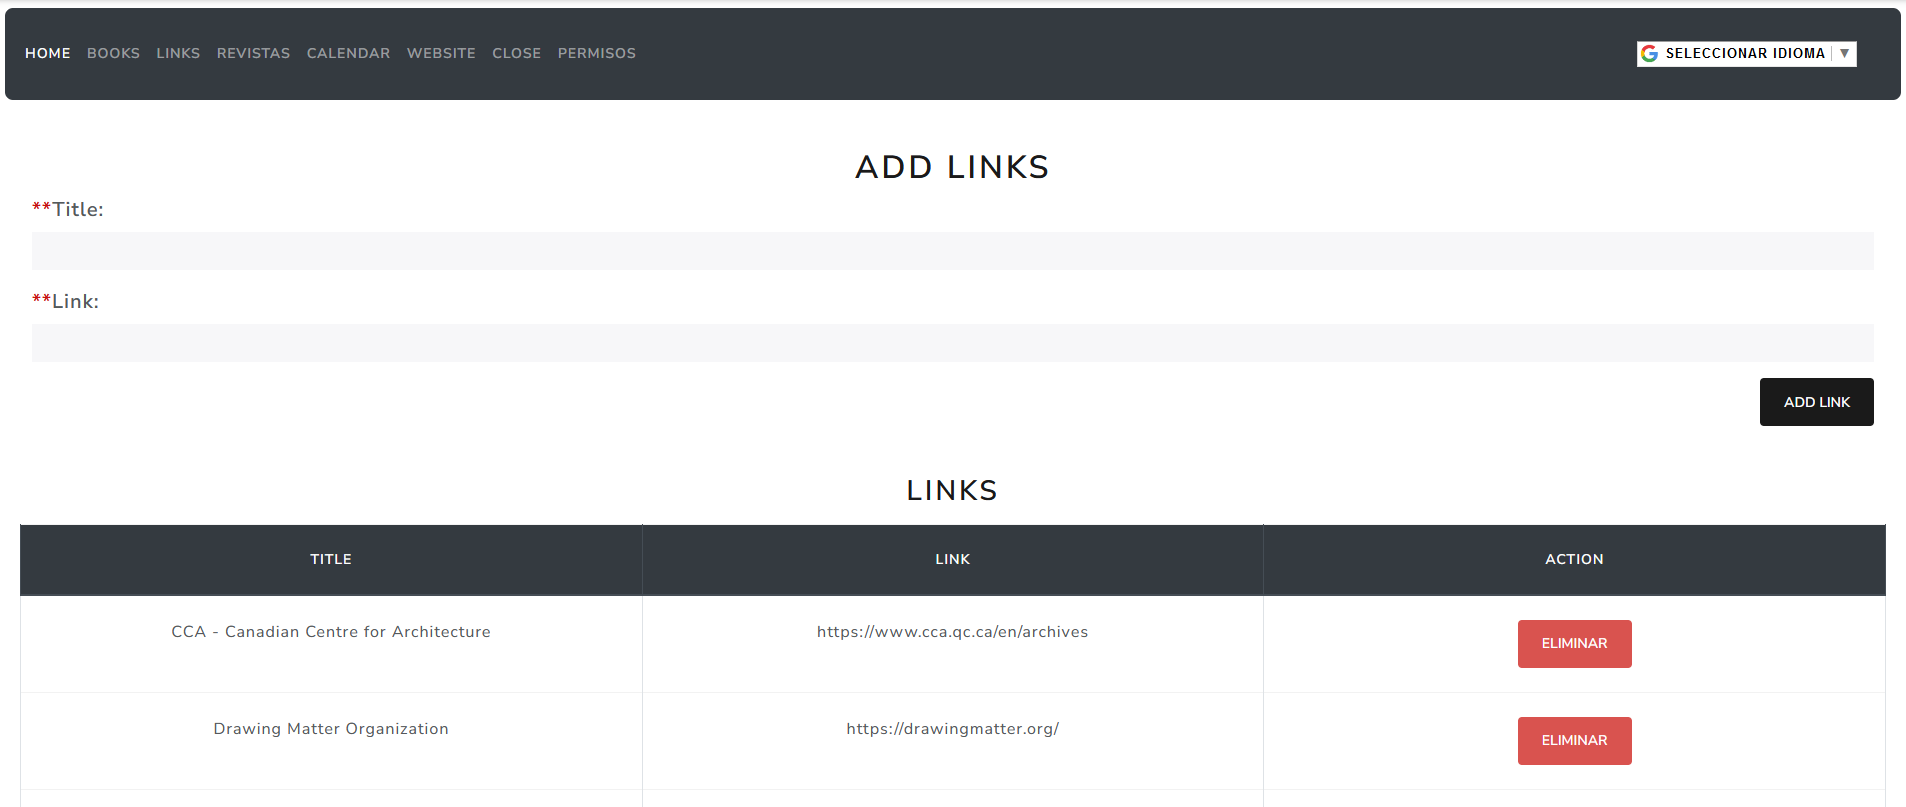
\includegraphics[width=0.7\textwidth]{img/linksadmin.png}
  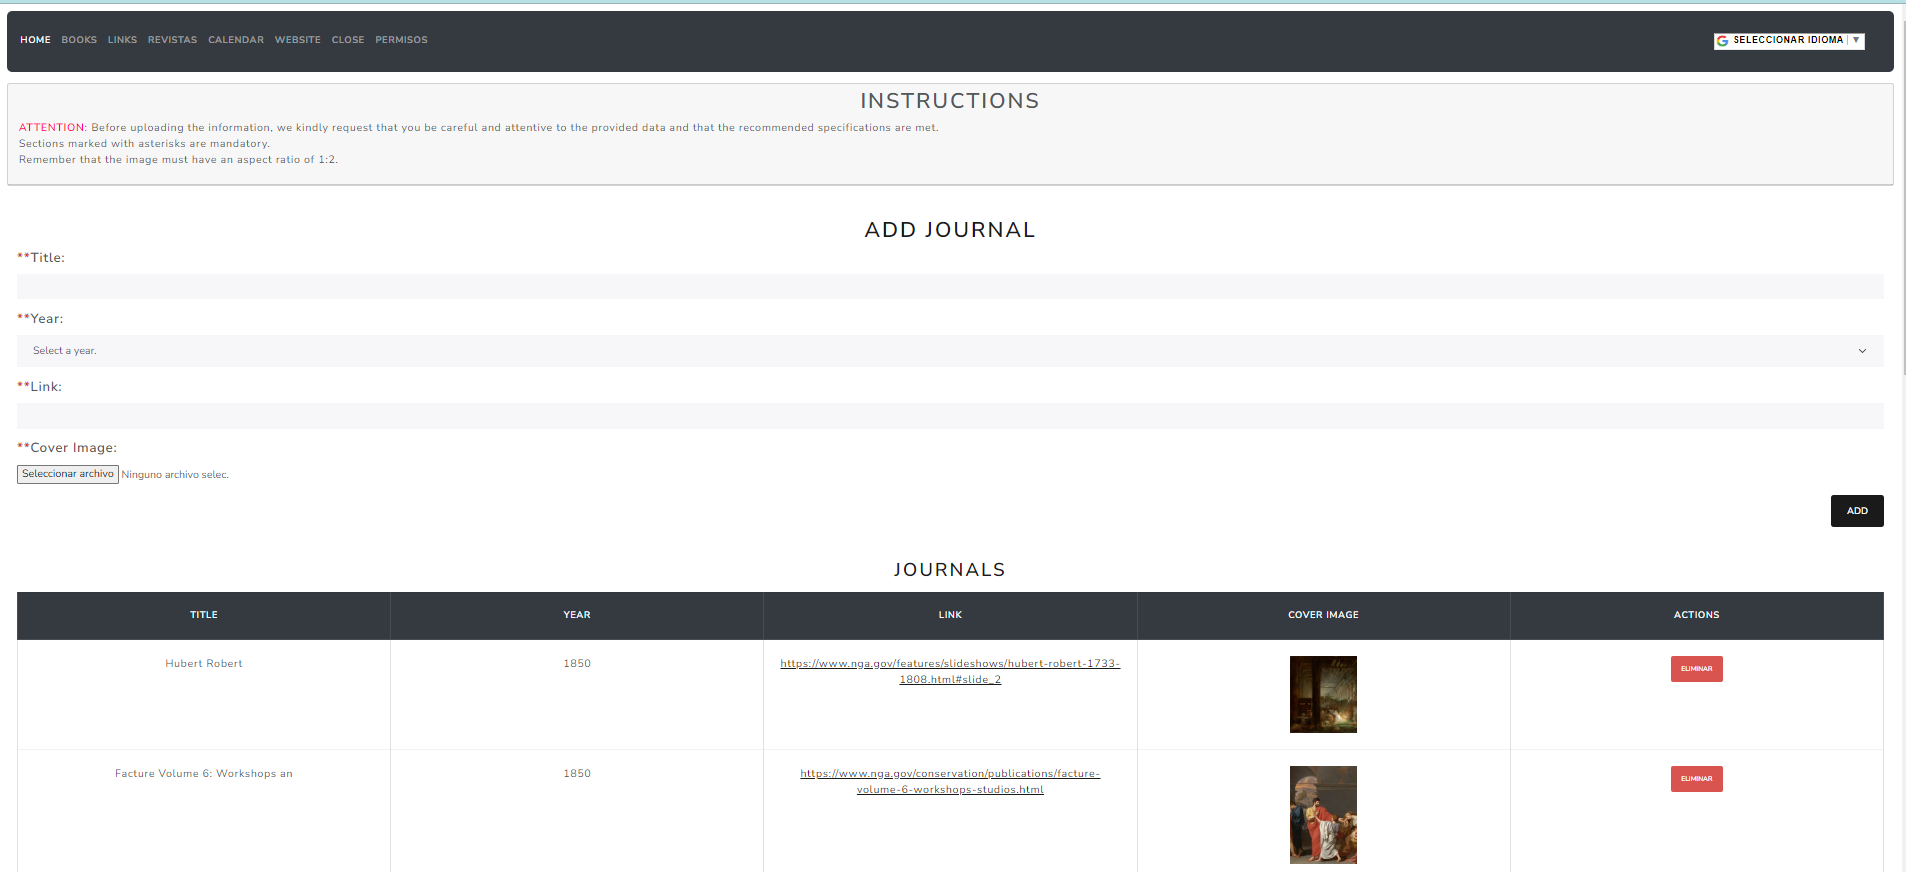
\includegraphics[width=0.7\textwidth]{img/linksadmin1.png}
  \caption{Links - Journals desde Administrador}
  \label{fig:journadmin}
\end{figure}

\subsection{Gestión de Libros: Publicar, Eliminar y Editar}
\label{sec:publish-delete-edit-books}

En esta fase de evaluación, nos centramos en las capacidades de la plataforma para la gestión de libros, abordando las operaciones de publicación, 
eliminación y edición. (ver Figura~\ref{fig:librosadminedit})

Primero, nos aseguramos de que los usuarios autorizados pudieran publicar nuevos libros de manera efectiva. Verificamos que el proceso de publicación 
fuera claro y accesible, permitiendo a los usuarios ingresar la información necesaria, como el título, el autor y la descripción del libro, de manera 
fluida y sin contratiempos.

Luego, evaluamos la función de eliminación para garantizar que los usuarios pudieran eliminar libros existentes según fuera necesario. Esta capacidad es 
esencial para mantener la plataforma actualizada y gestionar eficientemente el contenido disponible.

Por último, examinamos la función de edición para asegurar que los usuarios autorizados pudieran modificar la información de los libros de manera precisa 
y sin errores. Esto incluyó la capacidad de editar detalles como el título, el autor, la fecha, portada, añadir o elimiar imagenes, videos o pdf y la descripción 
del libro, asegurando que cualquier cambio realizado fuera coherente y válido.

En resumen, durante esta evaluación, confirmamos que la plataforma puede gestionar de manera efectiva la publicación, eliminación y edición de libros, 
proporcionando a los usuarios una experiencia sin complicaciones y garantizando la integridad del contenido mostrado.
\begin{figure}
  \centering
  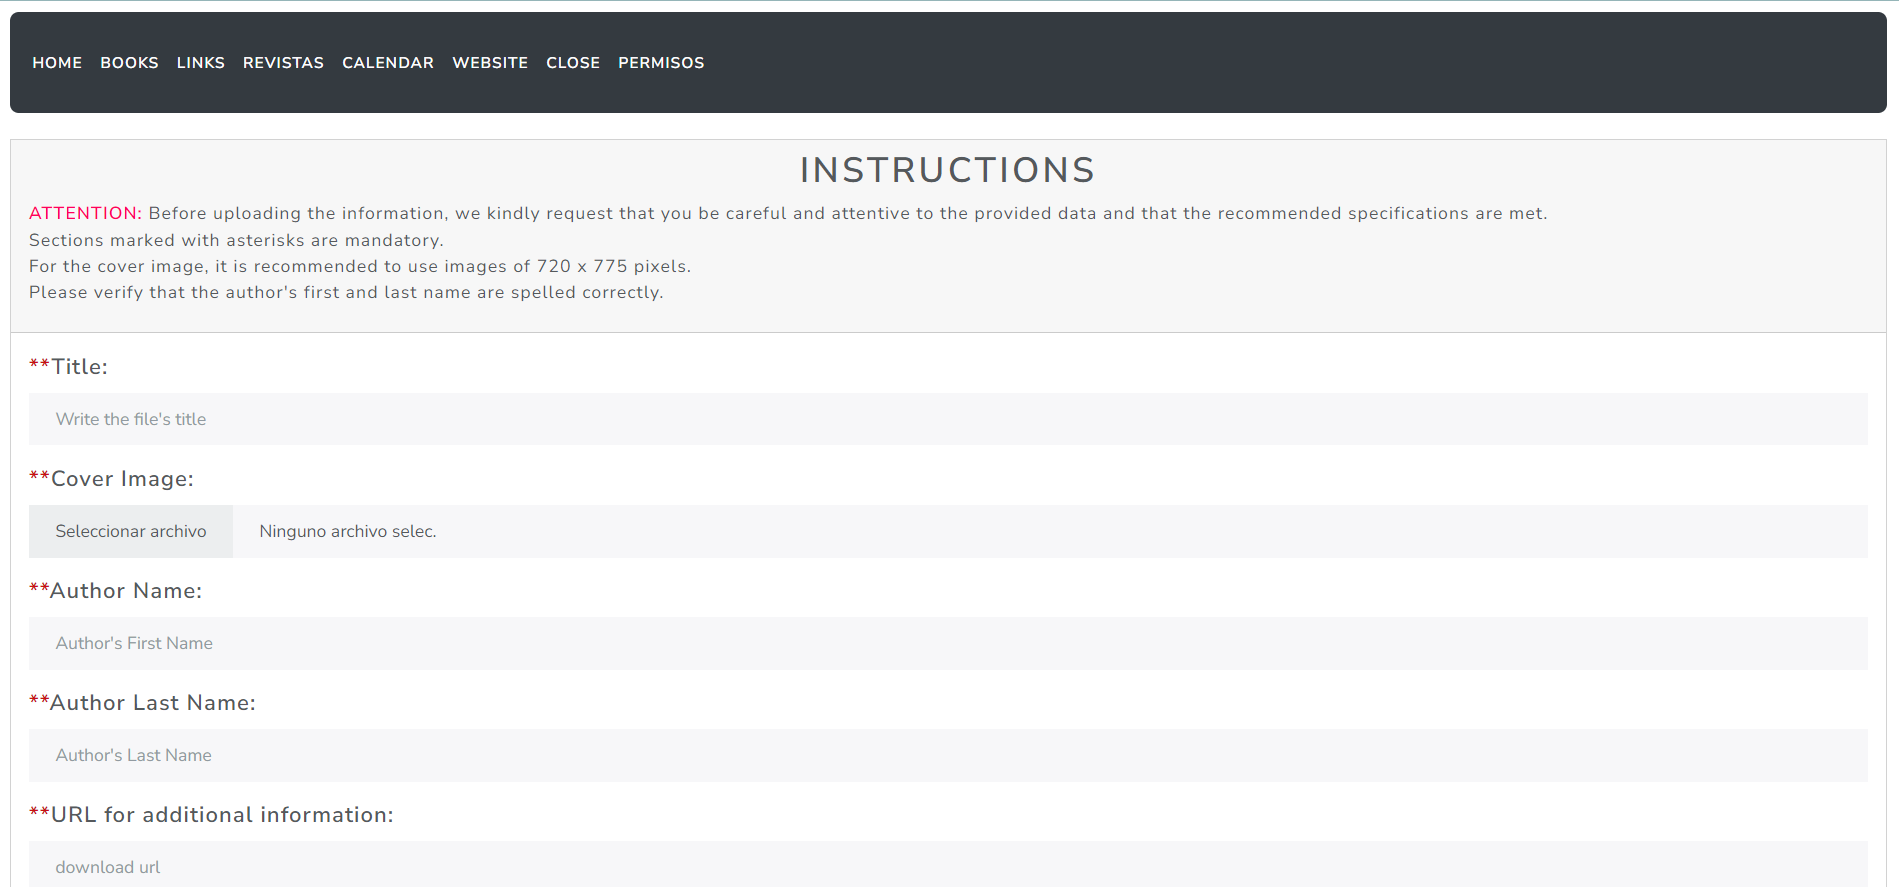
\includegraphics[width=0.7\textwidth]{img/booksadmin.png}
  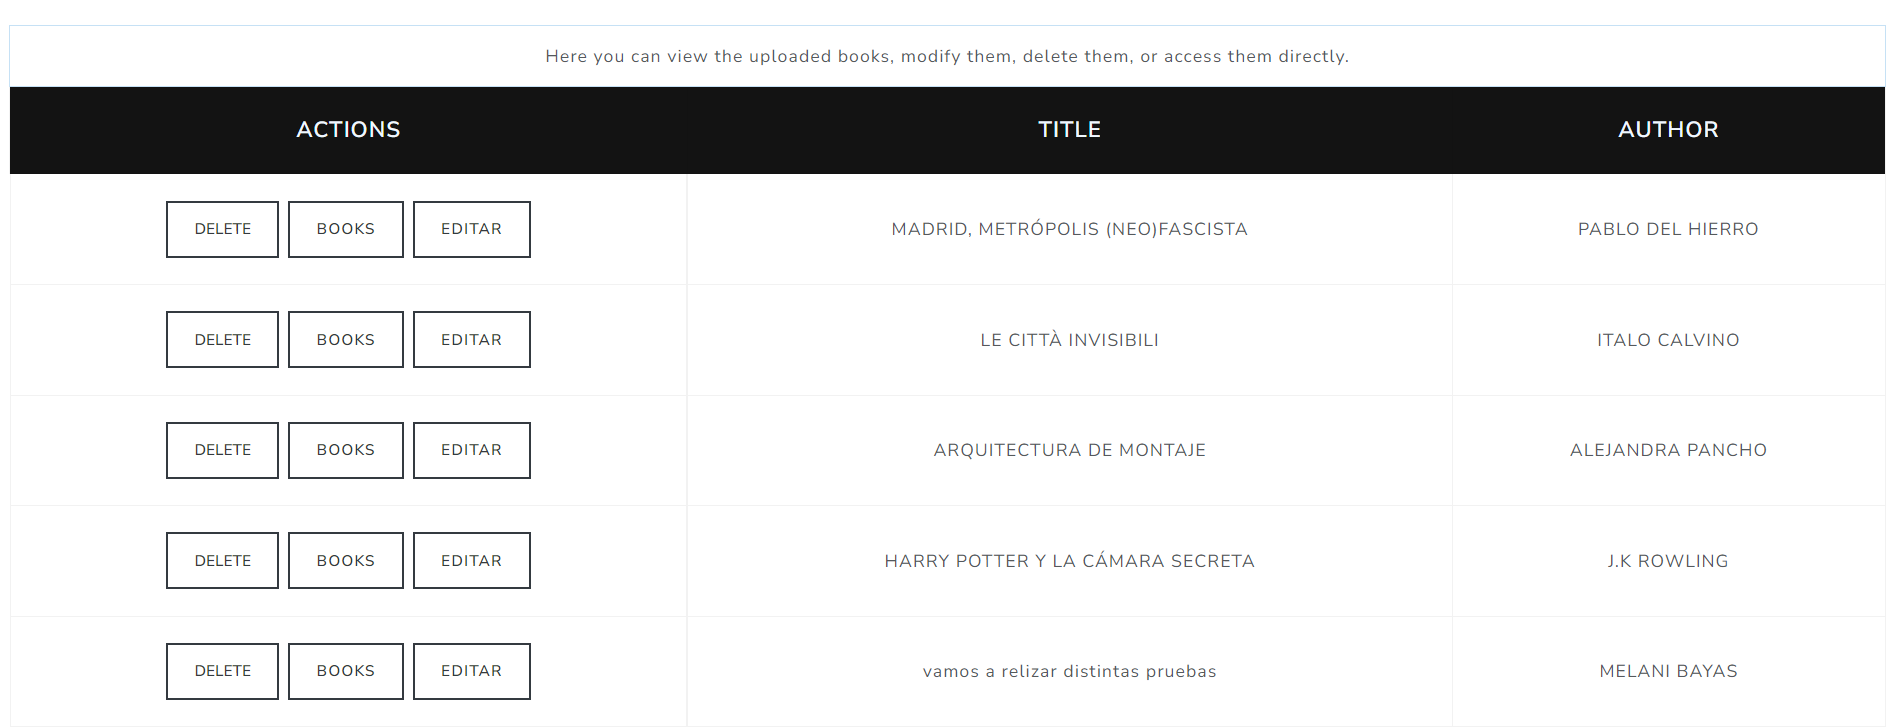
\includegraphics[width=0.7\textwidth]{img/booksadmin2.png}
  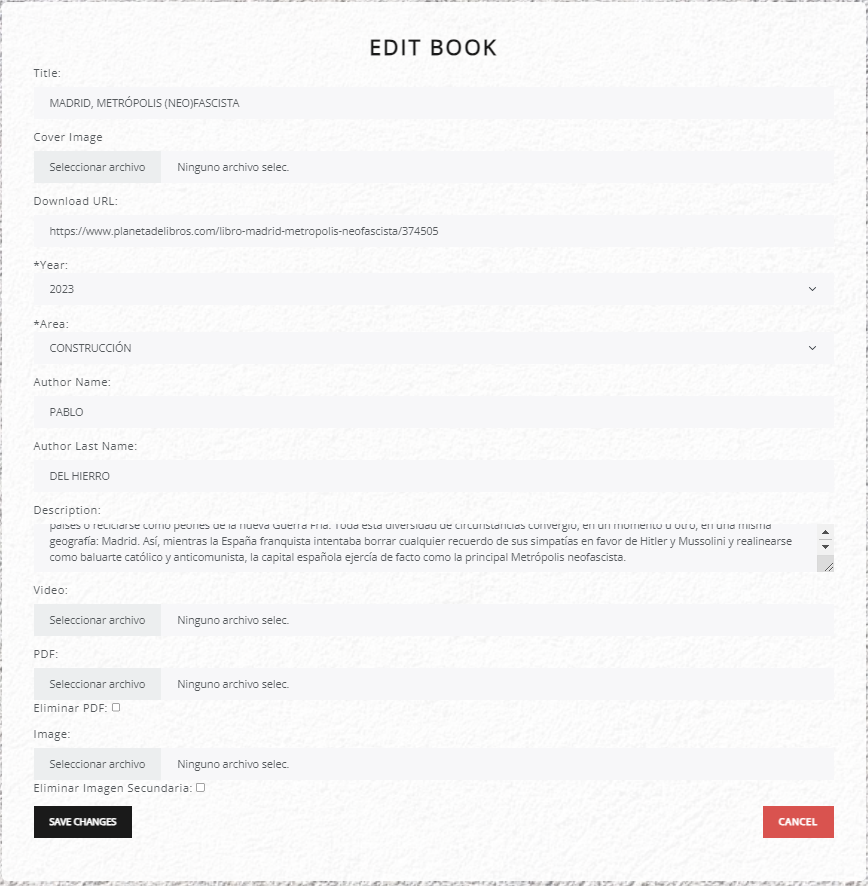
\includegraphics[width=0.7\textwidth]{img/booksadmin3.png}
  \caption{Books desde la vista admin}
  \label{fig:librosadminedit}
\end{figure}

\subsection{Comentar en Publicaciones}
\label{sec:comment-on-posts}

Durante esta evaluación, nos centramos en la capacidad de la plataforma para permitir a los usuarios comentar en las publicaciones. Verificamos que los usuarios 
autorizados pudieran agregar comentarios de manera efectiva los libros. Nos aseguramos de que el proceso de comentario fuera claro y accesible, permitiendo a los 
usuarios expresar sus opiniones y participar en discusiones de manera significativa. (ver Figura~\ref{fig:comentarios})

Además, evaluamos la funcionalidad de moderación de comentarios para garantizar que los administradores pudieran gestionar los comentarios de manera efectiva, 
incluida la capacidad de eliminar comentarios inapropiados o irrelevantes según fuera necesario.

En resumen, durante esta evaluación, confirmamos que la plataforma puede facilitar la interacción de los usuarios a través de comentarios en los libros, 
promoviendo la participación activa y la comunicación entre todos.

\begin{figure}
  \centering
  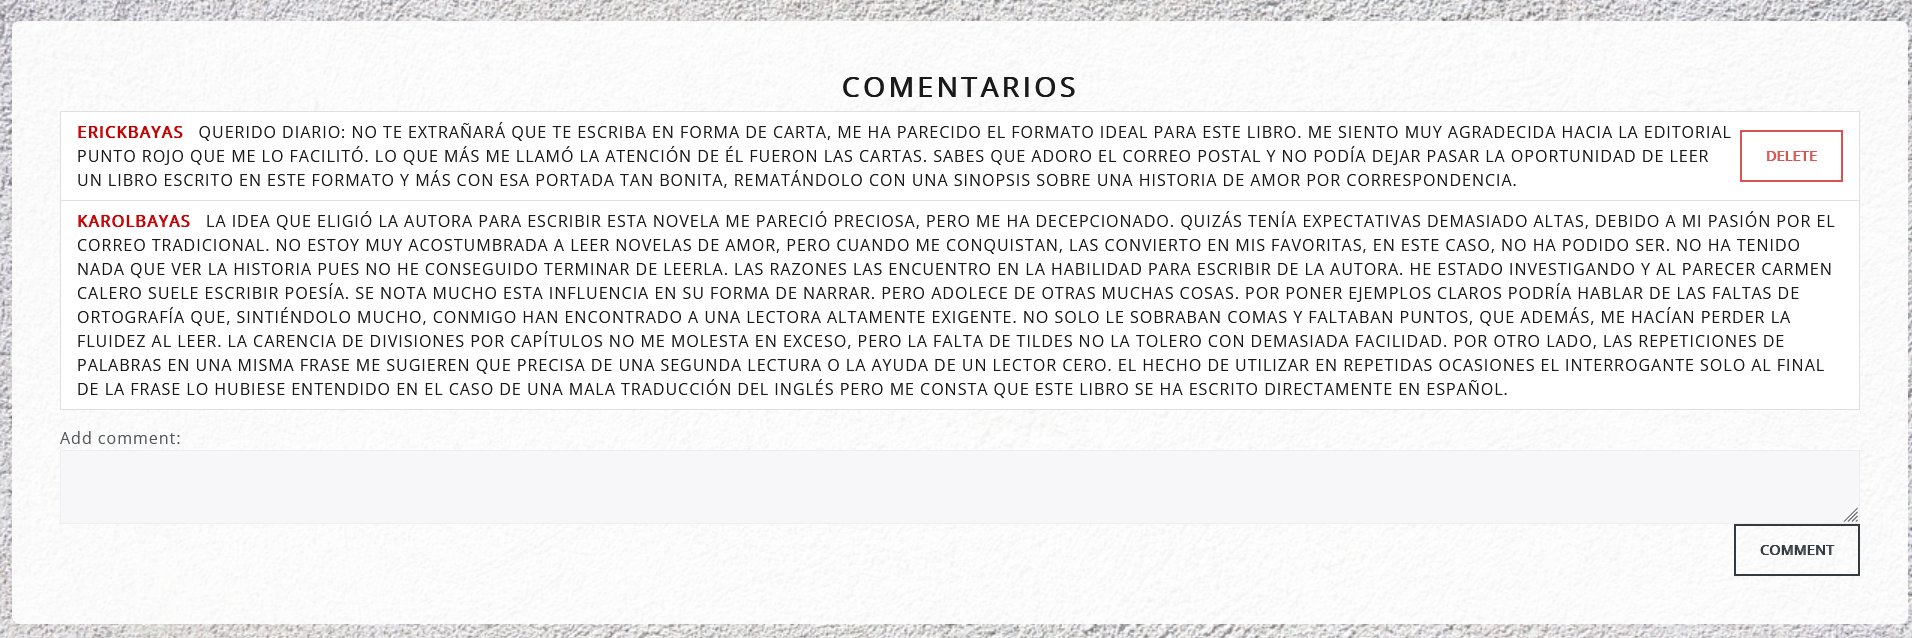
\includegraphics[width=0.7\textwidth]{img/comentarios.png}
  \caption{Vista de Comentarios desde el perfil de un alumno}
  \label{fig:comentarios}
\end{figure}
\subsection{Dar Permisos a Usuarios}
\label{sec:grant-permissions-users}

En esta fase de evaluación, nos centramos en la capacidad de la plataforma para administrar los permisos de los usuarios (Solo el administrador podra otorgar permisoa). 
Verificamos que los administradores pudieran asignar y gestionar los permisos de los usuarios de manera efectiva, controlando qué funciones y se pueda 
acceder con los usuarios en función de sus roles y privilegios. (ver Figura~\ref{fig:permisosadmin})

Nos aseguramos de que el proceso de asignación de permisos fuera claro y accesible, permitiendo a los administradores definir los roles de los usuarios y asignar 
permisos específicos de manera precisa y sin complicaciones.

Además, evaluamos la funcionalidad de control de acceso para garantizar que los usuarios solo pudieran acceder a las funciones y recursos para los que tienen los 
permisos adecuados, garantizando así la seguridad y la integridad de la plataforma.

En resumen, durante esta evaluación, confirmamos que la plataforma puede gestionar de manera efectiva los permisos de los usuarios, proporcionando un control 
granular sobre el acceso a las funciones y recursos, y garantizando la seguridad y la confidencialidad de la información.
\begin{figure}
  \centering
  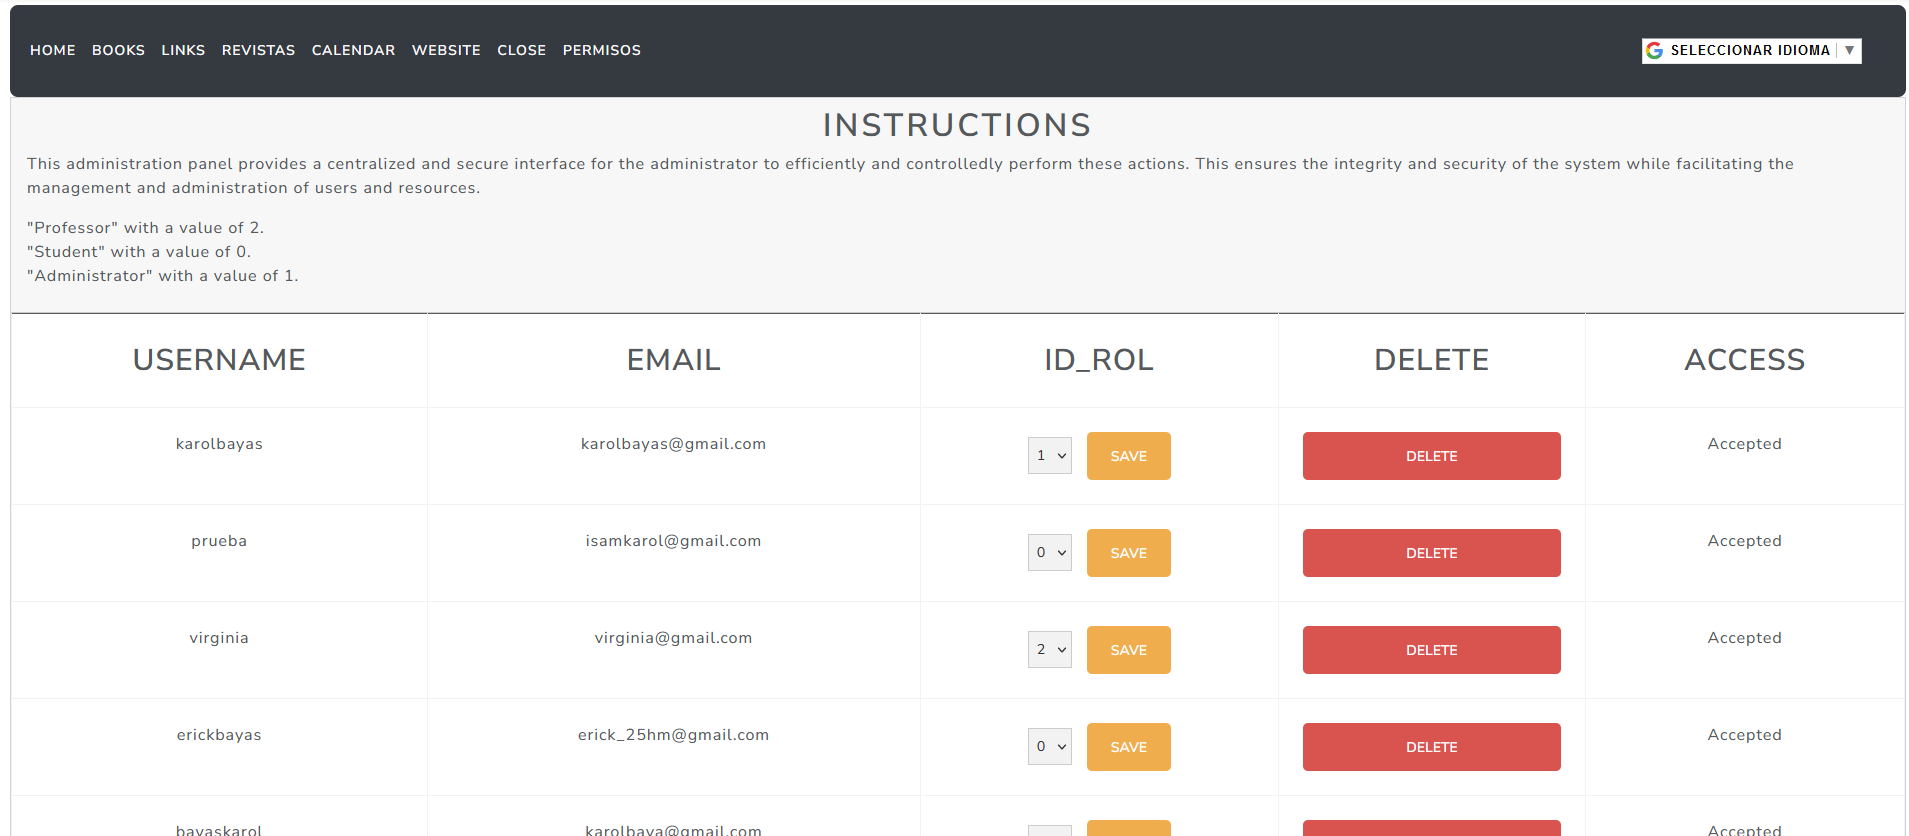
\includegraphics[width=0.7\textwidth]{img/permisos.png}
  \caption{Vista de Permisos desde el Administrador}
  \label{fig:permisosadmin}
\end{figure}

\section{Conclusiones de los resultados}
\label{sec:resultados}

Durante estas pruebas, se observó que los libros podían ser subidos y también editados para ajustar detalles como el título, el autor, el año, el área, la descripción 
entre otros datos. 
Además, se confirmó que la función de eliminación funcionaba de manera efectiva, permitiendo la eliminación exitosa de libros de la plataforma. Sin embargo, 
en el caso de los enlaces y las revistas, se constató que solo era posible cargarlos y eliminarlos, sin la opción de realizar ediciones en sus detalles.

Además, se realizó un análisis detallado para garantizar que los diferentes tipos de usuarios solo pudieran acceder a los elementos pertinentes y a los 
archivos que ellos mismos habían cargado. Por ejemplo, se verificó que los usuarios alumnos no pudieran acceder a las funciones de administración ni ver 
documentos subidos por otros usuarios que no estuvieran disponibles para el acceso público. Mientras tanto, los administradores tuvieron acceso y pudieron 
realizar operaciones en todos los archivos, independientemente de su origen.

Estos resultados validan la robustez de la plataforma y su capacidad para gestionar las operaciones necesarias de manera segura y eficiente, cumpliendo con los 
estándares y requisitos establecidos previamente.


%%%%%%%%%%%%%%%%%%%%%%%%%%%%%%%%%%%%%%%%%%%%%%%%%%%%%%%%%%%%%%%%%%%%%%%%%%%%%%%%
%%%%%%%%%%%%%%%%%%%%%%%%%%%%%%%%%%%%%%%%%%%%%%%%%%%%%%%%%%%%%%%%%%%%%%%%%%%%%%%%
% CONCLUSIONES %
%%%%%%%%%%%%%%%%%%%%%%%%%%%%%%%%%%%%%%%%%%%%%%%%%%%%%%%%%%%%%%%%%%%%%%%%%%%%%%%%

\cleardoublepage
\chapter{Conclusiones}
\label{chap:conclusiones}


\section{Conclusión del Proyecto}

Este proyecto ha sido una experiencia enriquecedora, enfocada en proporcionar una solución integral y satisfactoria para los usuarios, 
especialmente en el ámbito de la arquitectura. A lo largo de su desarrollo, hemos diseñado e implementado una plataforma versátil que 
cumple con las expectativas tanto de usuarios no registrados como de administradores del sistema.

Durante este proceso, nos hemos centrado en garantizar la calidad y la usabilidad del sistema. Realizamos pruebas exhaustivas en cada etapa 
del desarrollo para asegurarnos de que todas las funcionalidades, desde la validación de formularios hasta la gestión de usuarios, funcionen 
de manera óptima, brindando una experiencia fluida y sin problemas a los usuarios.

La inclusión de un panel de administración ha sido fundamental para permitir una gestión eficiente y controlada del sistema. Esto ha otorgado al 
administrador la capacidad de asignar roles, gestionar usuarios y controlar el acceso a diversas funcionalidades, lo que contribuye a la seguridad 
y la integridad del sistema en su conjunto.

En resumen, este proyecto representa un esfuerzo colaborativo y meticuloso orientado a satisfacer las necesidades y expectativas de los usuarios. 
A través de un diseño cuidadoso y una implementación diligente, hemos logrado crear un sistema que no solo cumple con los requisitos funcionales, 
sino que también ofrece una experiencia de usuario gratificante y satisfactoria.

\section{Aplicación de lo aprendido}
\label{sec:aplicacion}

La aplicación de los conocimientos y habilidades adquiridos durante mi formación en el Grado en Ingeniería en Sistemas Audiovisuales y Multimedia ha sido fundamental para la realización de este Trabajo de Fin de Grado. A continuación, mencionaré los aprendizajes que me permitieron llevar a cabo la extracción, tratamiento y clasificación de datos para realizar el análisis de este proyecto:

\begin{enumerate}
  \item \textbf{Informática I}: Esta asignatura me proporcionó las bases fundamentales de programación, sentando los cimientos necesarios para comprender y desarrollar código de manera efectiva.
  \item \textbf{Informática II}: En esta asignatura, además de reforzar mis conocimientos previos de programación, adquirí una formación más avanzada en herramientas comúnmente utilizadas en el desarrollo de software. Además, mejoré en la estructuración del código y en la lógica necesaria para la programación.
  \item \textbf{Protocolos para la Transmisión de Audio y Vídeo por Internet}: En este curso, obtuve conocimientos sobre el lenguaje de programación Python y aprendí cómo se estructura y para qué se utiliza la estructura de datos JSON. Estos conocimientos fueron fundamentales para la manipulación y tratamiento de datos en este proyecto.
  \item \textbf{Construcción de Servicios y Aplicaciones Audiovisuales en Internet}: En este curso, adquirí habilidades específicas relacionadas con la construcción de servicios y aplicaciones en el ámbito audiovisual en internet. Aprendí sobre los principios fundamentales y las tecnologías utilizadas en el desarrollo de servicios y aplicaciones multimedia en la web, lo que me proporcionó una base sólida para la implementación de funcionalidades relacionadas con el contenido audiovisual en este proyecto.
  \item \textbf{Laboratorio de Tecnologías Audiovisuales en la Web}: Durante este curso, tuve la oportunidad de aplicar los conocimientos teóricos adquiridos en la construcción práctica de aplicaciones y servicios multimedia en la web. A través de actividades de laboratorio y proyectos prácticos, desarrollé habilidades prácticas en el diseño, desarrollo y despliegue de tecnologías audiovisuales en entornos web. Estas habilidades fueron fundamentales para la implementación exitosa de funcionalidades multimedia en este proyecto.
\end{enumerate}

En resumen, la combinación de estos conocimientos y habilidades adquiridos a lo largo de mi formación académica me ha proporcionado las herramientas necesarias para llevar a cabo con éxito la elaboración de este Trabajo de Fin de Grado y realizar un análisis profundo y significativo del proyecto.


\section{Lecciones aprendidas}
\label{sec:lecciones_aprendidas}

Durante la realización de este proyecto, tuve la oportunidad de adquirir nuevos conocimientos y habilidades que no había explorado durante mi formación académica 
en la universidad. En particular, destacaría tres aspectos fundamentales:

\begin{enumerate}
  \item \textbf{Uso de Docker}: A través de este proyecto, aprendí a utilizar Docker, una herramienta de virtualización que facilita la creación, implementación y ejecución de aplicaciones en entornos aislados. Esta experiencia me permitió comprender mejor los conceptos relacionados con la virtualización y la gestión de contenedores, así como mejorar mis habilidades en el despliegue de aplicaciones en diferentes entornos.
  \item \textbf{Gestión de Base de Datos}: Durante la realización de este proyecto, adquirí experiencia en la gestión de bases de datos, incluyendo la creación de esquemas, la inserción y consulta de datos, y la optimización del rendimiento de las consultas. Esta experiencia fue fundamental para el desarrollo de funcionalidades relacionadas con el almacenamiento y recuperación de información en el sistema.
  \item \textbf{Uso del Framework Flask}: Uno de los aspectos más destacados de este proyecto fue aprender a utilizar el framework Flask para el desarrollo de aplicaciones web en Python. A través de la práctica y la experimentación, adquirí habilidades en el diseño y desarrollo de aplicaciones web dinámicas y escalables. El uso de Flask me permitió implementar funcionalidades complejas de manera eficiente y mantener una estructura organizada en el código del proyecto.
\end{enumerate}

En resumen, la realización de este proyecto me brindó la oportunidad de explorar y adquirir nuevos conocimientos y habilidades que 
no había tenido la oportunidad de desarrollar durante mi formación académica en la universidad. El aprendizaje de Docker, la gestión 
de bases de datos y el uso del framework Flask fueron aspectos fundamentales que enriquecieron mi experiencia y ampliaron mis horizontes en el campo de la ingeniería de sistemas audiovisuales y multimedia.

\section{Trabajos futuros}
\label{sec:trabajos_futuros}

Este proyecto no solo marca un hito en su estado actual, sino que también sienta las bases para futuros desarrollos y expansiones. 
Se pretende convertir esta aplicación en un proyecto a futuro, con la meta de alojarla en un servidor accesible para cualquier usuario. 
Además, se planifica ampliar su funcionalidad mediante la incorporación de nuevas características y tecnologías.

Entre los trabajos futuros planeados para esta aplicación se incluyen:

\begin{itemize}
  \item \textbf{Añadir redes neuronales mediante conectores}: Se explorará la posibilidad de integrar redes neuronales en la aplicación 
  mediante conectores especializados. Esto permitirá mejorar el análisis y la interpretación de datos, así como ofrecer funcionalidades 
  avanzadas basadas en inteligencia artificial.
  \item \textbf{Ampliar la gestión de bases de datos}: Se considerará la incorporación de la capacidad para administrar múltiples bases 
  de datos, lo que ofrecerá mayor flexibilidad y escalabilidad al sistema. Esto incluirá la posibilidad de trabajar con bases de datos 
  relacionales y no relacionales, según las necesidades específicas de los usuarios.
  \item \textbf{Innovar para convertirla en una plataforma completa}: Se buscará continuamente la innovación y el desarrollo de nuevas 
  funcionalidades para convertir esta aplicación en una plataforma completa que cumpla con todos los requisitos y necesidades de los 
  usuarios. Esto implica mantenerse al tanto de las últimas tendencias tecnológicas y adaptar la aplicación en consecuencia.
\end{itemize}

En resumen, se proyecta un futuro emocionante para esta aplicación, con la visión de convertirla en una herramienta robusta, versátil y completa que continúe creciendo y evolucionando para satisfacer las demandas cambiantes del mercado y las necesidades de los usuarios.



%%%%%%%%%%%%%%%%%%%%%%%%%%%%%%%%%%%%%%%%%%%%%%%%%%%%%%%%%%%%%%%%%%%%%%%%%%%%%%%%
%%%%%%%%%%%%%%%%%%%%%%%%%%%%%%%%%%%%%%%%%%%%%%%%%%%%%%%%%%%%%%%%%%%%%%%%%%%%%%%%
% APÉNDICE(S) %
%%%%%%%%%%%%%%%%%%%%%%%%%%%%%%%%%%%%%%%%%%%%%%%%%%%%%%%%%%%%%%%%%%%%%%%%%%%%%%%%

\cleardoublepage
\appendix
\chapter{Manual de usuario}
\label{app:manual}


\section{Bienvenida}
¡Bienvenido a nuestra aplicación! Este manual tiene como objetivo proporcionarte toda la información necesaria para utilizar nuestra 
plataforma de manera efectiva y segura.

\section{Registro de Usuario}

Para acceder a todas las funcionalidades de la aplicación, es necesario registrarse. Sigue estos pasos:

\begin{enumerate}
    \item Accede a la página de registro.
    \item Completa el formulario con tu dirección de correo electrónico y un nombre de usuario único.
    \item Una vez registrado, recibirás un correo electrónico de validación. Sigue las instrucciones para activar tu cuenta.
\end{enumerate}

Recuerda que cada cuenta solo puede tener una dirección de correo electrónico y un nombre de usuario únicos. El acceso a la aplicación 
será otorgado por el administrador.

\section{Inicio de Sesión}

Una vez que tu cuenta esté activada, puedes iniciar sesión en la aplicación:

\begin{enumerate}
    \item Ingresa tu correo electrónico y contraseña en el formulario de inicio de sesión.
    \item Si olvidaste tu contraseña, puedes solicitar una nueva. Se te enviará un enlace único a tu correo electrónico para 
    restablecerla.
\end{enumerate}

\section{Gestión de Archivos}

Una vez dentro de la aplicación, podrás gestionar tus archivos subidos y compartidos de la siguiente manera:

\begin{itemize}
    \item En la sección de libros, podrás editar la información rellenando todos los campos requeridos. También podrás eliminar 
    documentos como videos, PDF y la foto extra si no es necesario.
    \item Los enlaces y revistas no son editables y siempre deben tener todos los datos rellenados. Si por algun motivo algún datos es 
    erroneo podrás eliminarlos y volvel a crearlos.
\end{itemize}

\section{Calendario}

Utiliza el calendario para programar eventos, reuniones y fechas importantes:

\begin{itemize}
    \item Solo los profesores y administradores pueden editar y eliminar eventos del calendario. Los alumnos solo pueden crear eventos.
\end{itemize}

\section{Comentarios}

Los comentarios en la aplicación están sujetos a las siguientes reglas:

\begin{itemize}
    \item Los comentarios pueden ser gestionados solo por usuarios registrados. Los administradores tienen la capacidad de eliminar comentarios inapropiados.
\end{itemize}

\section{Contacto}

Si tienes alguna pregunta o problema técnico, no dudes en ponerte en contacto. Envía un correo electrónico a karolbayas@gmail.com 
estare encantada de poder ayudarte a resolver tus dudas.

¡Gracias por utilizar nuestra aplicación!



%%%%%%%%%%%%%%%%%%%%%%%%%%%%%%%%%%%%%%%%%%%%%%%%%%%%%%%%%%%%%%%%%%%%%%%%%%%%%%%%
%%%%%%%%%%%%%%%%%%%%%%%%%%%%%%%%%%%%%%%%%%%%%%%%%%%%%%%%%%%%%%%%%%%%%%%%%%%%%%%%
% BIBLIOGRAFIA %
%%%%%%%%%%%%%%%%%%%%%%%%%%%%%%%%%%%%%%%%%%%%%%%%%%%%%%%%%%%%%%%%%%%%%%%%%%%%%%%%


\cleardoublepage

% Las siguientes dos instrucciones es todo lo que necesitas
% para incluir las citas en la memoria
\cleardoublepage
\bibliographystyle{abbrv}
\bibliography{memoria} 
 % memoria.bib es el nombre del fichero que contiene
% las referencias bibliográficas. Abre ese fichero y mira el formato que tiene,
% que se conoce como BibTeX. Hay muchos sitios que exportan referencias en
% formato BibTeX. Prueba a buscar en http://scholar.google.com por referencias
% y verás que lo puedes hacer de manera sencilla.
% Más información: 
% http://texblog.org/2014/04/22/using-google-scholar-to-download-bibtex-citations/

\end{document}
